% !TeX program = xelatex
\documentclass[12pt,a4paper]{report}

% ============================================================
% PENGATURAN BAHASA DAN FONT
% ============================================================
\usepackage[indonesian]{babel}
\usepackage{fontspec}
\setmainfont{Times New Roman}
\usepackage{unicode-math}
\setmathfont{TeX Gyre Termes Math}
\setmathfont[version=bold,FakeBold=2]{TeX Gyre Termes Math}

% ============================================================
% TATA LETAK DAN FORMAT DOKUMEN
% ============================================================
\usepackage{geometry}
\geometry{
    a4paper,
    left=4cm,
    right=3cm,
    top=3cm,
    bottom=3cm
}
\usepackage{setspace}
\usepackage{titlesec}
\usepackage{tocloft}

% ============================================================
% GAMBAR, TABEL, PERSAMAAN, DAN DIAGRAM
% ============================================================
\usepackage{graphicx}
\usepackage[table]{xcolor}
\usepackage{array}
\usepackage{tabularx}
\usepackage{multirow}
\usepackage{makecell}
\usepackage{caption}
\captionsetup{
    labelfont=bf,
    textfont=normalfont,
    labelsep=space
}
\renewcommand{\theadfont}{\bfseries}
\renewcommand{\theadalign}{cc}
\usepackage{amsmath}
\setcounter{MaxMatrixCols}{13}
\usepackage{tikz}
\usetikzlibrary{calc,arrows.meta}

% ============================================================
% SITASI, DAFTAR PUSTAKA, DAN TAUTAN
% ============================================================
\usepackage[numbers,sort&compress]{natbib}
\usepackage[hidelinks,linktoc=all]{hyperref}

% ============================================================
% FORMAT JUDUL DAN PENOMORAN
% ============================================================
\renewcommand{\thechapter}{\Roman{chapter}}
\renewcommand{\thesection}{\arabic{chapter}.\arabic{section}}
\renewcommand{\thesubsection}{\arabic{chapter}.\arabic{section}.\arabic{subsection}}
\renewcommand{\thesubsubsection}{\arabic{chapter}.\arabic{section}.\arabic{subsection}.\arabic{subsubsection}}
\renewcommand{\thefigure}{\arabic{chapter}.\arabic{figure}}
\renewcommand{\thetable}{\arabic{chapter}.\arabic{table}}
\numberwithin{equation}{chapter}
\renewcommand{\theequation}{\arabic{chapter}.\arabic{equation}}
\titleformat{\chapter}[display]
    {\normalfont\fontsize{14pt}{16pt}\selectfont\bfseries\centering}
    {\MakeUppercase{\chaptertitlename}\ \thechapter}
    {10pt}
    {\fontsize{14pt}{16pt}\selectfont}
\titlespacing*{\chapter}{0pt}{-20pt}{20pt}
\titleformat{\section}
    {\normalfont\fontsize{12pt}{14pt}\selectfont\bfseries}
    {\thesection}
    {1em}
    {}

% ============================================================
% FORMAT DAFTAR ISI, DAFTAR GAMBAR, DAN DAFTAR TABEL
% ============================================================
\AtBeginDocument{%
  \renewcommand{\contentsname}{DAFTAR ISI}%
  \renewcommand{\listfigurename}{DAFTAR GAMBAR}%
  \renewcommand{\listtablename}{DAFTAR TABEL}%
}
\renewcommand{\cftchapleader}{\cftdotfill{\cftdotsep}}
\renewcommand{\cftchapdotsep}{\cftdotsep}
\renewcommand{\cftdotsep}{1}
\setlength{\cftbeforechapskip}{2pt}
\setlength{\cftbeforetoctitleskip}{-20pt}
\setlength{\cftbeforeloftitleskip}{-20pt}
\setlength{\cftbeforelottitleskip}{-20pt}
\setlength{\cftaftertoctitleskip}{20pt}
\setlength{\cftafterloftitleskip}{20pt}
\setlength{\cftafterlottitleskip}{20pt}
\renewcommand{\cfttoctitlefont}{\hfill\fontsize{14pt}{16pt}\selectfont\bfseries}
\renewcommand{\cftaftertoctitle}{\hfill\mbox{}\par}
\renewcommand{\cftloftitlefont}{\hfill\fontsize{14pt}{16pt}\selectfont\bfseries}
\renewcommand{\cftafterloftitle}{\hfill\mbox{}\par}
\renewcommand{\cftlottitlefont}{\hfill\fontsize{14pt}{16pt}\selectfont\bfseries}
\renewcommand{\cftafterlottitle}{\hfill\mbox{}\par}

\begin{document}

% Mengatur jarak antarbaris menjadi 1,5 spasi.
\onehalfspacing

% ==========================================
% SAMPUL
% ==========================================
\begin{titlepage}
    \centering
    \vspace*{1cm}
    
    {\fontsize{14pt}{16pt}\selectfont\bfseries
    IMPLEMENTASI FISIK DAN EVALUASI \textit{EVENT-BASED RECONFIGURATION CONTROL} PADA SISTEM FORMASI ADAPTIF TERDESENTRALISASI KAWANAN \textit{QUADCOPTER} DI RUANG SEMPIT\par}
    
    \vspace{2.0cm}
    {\large \bfseries PROPOSAL TESIS\par}
    \vspace{1.5cm}
    
    
\includegraphics[width=3cm]{figures/logo_itb.png}\par
    
    \vspace{1.5cm}
    Oleh\par
    \vspace{0.5cm}
    {\large \bfseries Izma Alhazmi Herdian}\par
    {\large \bfseries 23825301}\par
    
    \vfill
    
    {\large \bfseries 
    MAGISTER INSTRUMENTASI DAN KONTROL\par
    FAKULTAS TEKNOLOGI INDUSTRI\par
    INSTITUT TEKNOLOGI BANDUNG\par
    2026\par}
\end{titlepage}

% Penomoran romawi untuk halaman depan
\pagenumbering{roman}
\setcounter{page}{1}

% ==========================================
% ABSTRAK
% ==========================================
\chapter*{ABSTRAK}
\addcontentsline{toc}{chapter}{ABSTRAK}

\begin{center}
    \textbf{IMPLEMENTASI FISIK DAN EVALUASI \textit{EVENT-BASED RECONFIGURATION CONTROL} PADA SISTEM FORMASI ADAPTIF TERDESENTRALISASI KAWANAN \textit{QUADCOPTER} DI RUANG SEMPIT}

    \vspace{0.8cm}
    Oleh\\
    \textbf{Izma Alhazmi Herdian}\\
    23825301

    \vspace{0.8cm}
    (Program Studi Instrumentasi dan Kontrol)
\end{center}

\vspace{0.8cm}

\noindent
Navigasi kawanan \textit{quadcopter} di ruang sempit membutuhkan sistem kontrol formasi yang adaptif. Penelitian ini mengimplementasikan dan mengevaluasi sistem kontrol desentralisasi formasi adaptif menggunakan \textit{Event-Based Reconfiguration Control} (ERC\label{abbr:erc}) pada perangkat keras fisik. Setiap agen mempertahankan formasi secara mandiri dan melakukan rekonfigurasi otonom saat menghadapi penyempitan ruang. Melalui mekanisme berbasis kejadian, manuver adaptasi hanya terpicu saat parameter persepsi lingkungan melewati ambang batas, sehingga efisiensi komputasi dan \textit{bandwidth} komunikasi jaringan meningkat secara signifikan.

\noindent
Evaluasi eksperimental berfokus pada kestabilan formasi, akurasi pelacakan lintasan, dan ketahanan (\textit{robustness}) sistem terhadap kendala fisik dunia nyata, khususnya latensi komunikasi nirkabel dan derau (\textit{noise}) sensor lokalisasi \textit{indoor}. Hasil penelitian ini diharapkan dapat memvalidasi keandalan algoritma ERC secara empiris, menghasilkan rancangan sistem kontrol multi-agen yang terukur, tangguh, dan jauh lebih fleksibel dibandingkan metode formasi statis konvensional.

\vspace{1cm}
\noindent \textbf{Kata kunci:} quadcopter, kontrol desentralisasi, formasi adaptif, \textit{event-based reconfiguration control}, navigasi kawanan.

% ==========================================
% ABSTRACT
% ==========================================
\chapter*{ABSTRACT}
\addcontentsline{toc}{chapter}{ABSTRACT}

\begin{center}
    \textbf{PHYSICAL IMPLEMENTATION AND EVALUATION OF \textit{EVENT-BASED RECONFIGURATION CONTROL} FOR DECENTRALIZED ADAPTIVE FORMATION OF QUADCOPTER SWARMS IN NARROW SPACES}

    \vspace{0.8cm}
    By\\
    \textbf{Izma Alhazmi Herdian}\\
    23825301

    \vspace{0.8cm}
    (Instrumentation and Control Study Program)
\end{center}

\vspace{0.8cm}

\noindent
Navigating quadcopter swarms in narrow environments requires an adaptive formation control system. This research implements and evaluates a decentralized adaptive formation control system using \textit{Event-Based Reconfiguration Control} (ERC) on physical hardware. Each agent maintains formation independently and performs autonomous reconfiguration when encountering spatial constraints. Through an event-based mechanism, adaptation maneuvers are triggered only when environmental perception parameters cross specific thresholds, significantly improving computational and communication \textit{bandwidth} efficiency.

\noindent
The experimental evaluation focuses on formation stability, trajectory tracking accuracy, and system robustness against real-world physical constraints, specifically wireless communication latency and indoor localization sensor noise. The expected result of this research is the empirical validation of the ERC algorithm, yielding a scalable, robust, and much more flexible multi-agent control system design compared to conventional static formation methods.

\vspace{1cm}
\noindent \textbf{Keywords:} quadcopter, decentralized control, adaptive formation, \textit{event-based reconfiguration control}, swarm navigation.

% ==========================================
% HALAMAN PENGESAHAN
% ==========================================
\chapter*{HALAMAN PENGESAHAN}
\addcontentsline{toc}{chapter}{HALAMAN PENGESAHAN}

\begin{center}
    \textbf{IMPLEMENTASI FISIK DAN EVALUASI \textit{EVENT-BASED RECONFIGURATION CONTROL} PADA SISTEM FORMASI ADAPTIF TERDESENTRALISASI KAWANAN \textit{QUADCOPTER} DI RUANG SEMPIT}

    \vspace{0.8cm}
    Oleh\\
    \textbf{Izma Alhazmi Herdian}\\
    NIM: 23825301

    \vspace{0.8cm}
    (Program Studi Instrumentasi dan Kontrol)

    \vspace{0.8cm}
    Institut Teknologi Bandung

    \vspace{1.5cm}
    Menyetujui\\
    Tim Pembimbing

    \vspace{0.8cm}
    Tanggal 17 Agustus 2026
\end{center}

\vspace{1.2cm}

\noindent
\begin{minipage}[t]{0.49\textwidth}
    \centering
    Pembimbing 1

    \vspace{2.5cm}

    {\bfseries Ir. Estiyanti Ekawati, M.T., Ph.D.}\\
    NIP. 19690805 200801 2 020
\end{minipage}
\hfill
\begin{minipage}[t]{0.49\textwidth}
    \centering
    Pembimbing 2

    \vspace{2.5cm}

    {\bfseries Faqihza Mukhlish, S.T., M.T., Ph.D.}\\
    NIP. 121110001 
\end{minipage}

% ==========================================
% KATA PENGANTAR
% ==========================================
\chapter*{KATA PENGANTAR}
\addcontentsline{toc}{chapter}{KATA PENGANTAR}

Segala puji dan syukur penulis panjatkan ke hadirat Allah Swt. atas rahmat dan hidayah-Nya, sehingga penulis dapat menyelesaikan proposal tesis yang berjudul ``Implementasi Fisik dan Evaluasi \textit{Event-Based Reconfiguration Control} pada Sistem Formasi Adaptif Terdesentralisasi Kawanan \textit{Quadcopter} di Ruang Sempit''. Proposal tesis ini disusun sebagai bagian dari pemenuhan syarat akademik untuk memperoleh gelar Magister di Program Studi Instrumentasi dan Kontrol, Fakultas Teknologi Industri, Institut Teknologi Bandung. Penulis berharap bahwa proposal ini dapat menjadi landasan dalam perancangan sistem kontrol desentralisasi formasi adaptif untuk navigasi kawanan quadcopter serta memberikan referensi bagi pengembangan lebih lanjut di bidang terkait.

Penulis menyadari sepenuhnya bahwa penyusunan proposal tesis ini tidak mungkin terwujud tanpa bimbingan, dukungan, dan bantuan dari berbagai pihak. Oleh karena itu, penghargaan dan rasa terima kasih yang sebesar-besarnya disampaikan kepada:

\begin{enumerate}
    \item Ir. Estiyanti Ekawati, M.T., Ph.D., selaku dosen pembimbing pertama yang telah memberikan bimbingan, arahan, masukan teknis, serta metodologi penelitian yang sangat berharga selama proses pengerjaan tesis ini.
    \item Faqihza Mukhlish, S.T., M.T., Ph.D., selaku dosen pembimbing kedua yang telah memberikan bimbingan, arahan, masukan, serta bantuan dalam memecahkan permasalahan teknis yang dihadapi selama penelitian.
    \item Seluruh dosen dan tenaga kependidikan di Program Studi Instrumentasi dan Kontrol, atas dukungan dalam berbagai aspek akademik serta bantuan dalam hal administratif.
    \item Rekan-rekan di Pusat Teknologi, Instrumentasi, dan Otomasi, atas dukungan, diskusi, dan pertukaran gagasan selama proses penelitian.
    \item Kedua orang tua penulis yang senantiasa memberikan doa, semangat, serta dukungan moral, materiil, dan motivasi yang tiada henti.
    \item Seluruh pihak yang telah membantu dalam berbagai bentuk, baik secara langsung maupun tidak langsung, yang tidak dapat disebutkan satu per satu.
\end{enumerate}

Penulisan proposal ini masih jauh dari kesempurnaan dan memiliki berbagai keterbatasan, baik dalam hal substansi maupun penyajiannya. Oleh karena itu, penulis sangat mengharapkan kritik dan saran yang membangun agar proposal ini dapat disempurnakan serta menjadi lebih baik di masa mendatang.

\vspace{1cm}
\begin{flushright}
    Bandung, 17 Agustus 2026\\[1.8cm]
    Penulis
\end{flushright}

% ==========================================
% DAFTAR ISI, GAMBAR, TABEL, SINGKATAN
% ==========================================
\clearpage
\tableofcontents
\clearpage

\clearpage
\addcontentsline{toc}{chapter}{DAFTAR GAMBAR}
\listoffigures
\clearpage

\clearpage
\addcontentsline{toc}{chapter}{DAFTAR TABEL}
\listoftables
\clearpage

\chapter*{DAFTAR SINGKATAN DAN LAMBANG}
\addcontentsline{toc}{chapter}{DAFTAR SINGKATAN DAN LAMBANG}

\noindent
Daftar singkatan dan lambang yang digunakan dalam proposal ini disusun secara alfabetis untuk memudahkan pembaca dalam memahami istilah teknis, variabel, dan parameter yang muncul pada pembahasan.

\vspace{0.5cm}
\noindent\textbf{Daftar Singkatan}

\vspace{0.3cm}
\noindent\begin{tabularx}{\textwidth}{|>{\bfseries}p{2.4cm}|X|>{\centering\arraybackslash}p{1.8cm}|}
    \hline
    \rowcolor{gray!20}
    \thead{Singkatan} & \thead{Keterangan} & \thead{Hal.} \\ \hline
    CC & \textit{Companion Computer} & \pageref{abbr:cc} \\ \hline
    EKF & \textit{Extended Kalman Filter} & \pageref{abbr:ekf} \\ \hline
    ERC & \textit{Event-Based Reconfiguration Control} & \pageref{abbr:erc} \\ \hline
    ESC & \textit{Electronic Speed Controller} & \pageref{abbr:esc} \\ \hline
    FC & \textit{Flight Controller} & \pageref{abbr:fc} \\ \hline
    HITL & \textit{Hardware-In-The-Loop} & \pageref{abbr:hitl} \\ \hline
    IAPF & \textit{Improved Artificial Potential Field} & \pageref{abbr:iapf} \\ \hline
    MAVLink & \textit{Micro Air Vehicle Link} & \pageref{abbr:mavlink} \\ \hline
    PID & \textit{Proportional-Integral-Derivative} & \pageref{abbr:pid} \\ \hline
    PTIO & Pusat Teknologi Instrumentasi dan Otomasi & \pageref{abbr:ptio} \\ \hline
    RAB & Rencana Anggaran Biaya & \pageref{abbr:rab} \\ \hline
    RMSE & \textit{Root Mean Square Error} & \pageref{abbr:rmse} \\ \hline
    UAV & \textit{Unmanned Aerial Vehicle} & \pageref{abbr:uav} \\ \hline
    UDP & \textit{User Datagram Protocol} & \pageref{abbr:udp} \\ \hline
    UWB & \textit{Ultra-Wideband} & \pageref{abbr:uwb} \\ \hline
\end{tabularx}

\clearpage
\noindent\textbf{Daftar Lambang}

\vspace{0.3cm}
\noindent\begin{tabularx}{\textwidth}{|>{\centering\arraybackslash\bfseries}p{3cm}|X|>{\centering\arraybackslash}p{1.8cm}|}
    \hline
    \rowcolor{gray!20}
    \thead{Lambang} & \thead{Keterangan} & \thead{Hal.} \\ \hline
    $d_l$ & Jarak lateral antara sisi kiri wahana dan dinding atau rintangan kiri. & \pageref{sym:dl} \\ \hline
    $d_r$ & Jarak lateral antara sisi kanan wahana dan dinding atau rintangan kanan. & \pageref{sym:dr} \\ \hline
    $\phi$ (\textit{phi}) & Sudut rotasi \textit{roll} pada dinamika \textit{quadcopter}. & \pageref{sym:phi} \\ \hline
    $\psi$ (\textit{psi}) & Sudut rotasi \textit{yaw} pada dinamika \textit{quadcopter}. & \pageref{sym:psi} \\ \hline
    $\theta$ (\textit{theta}) & Sudut rotasi \textit{pitch} pada dinamika \textit{quadcopter}. & \pageref{sym:theta} \\ \hline
    $w_{\mathrm{body}}$ & Lebar fisik badan wahana quadcopter. & \pageref{sym:wbody} \\ \hline
    $w_e$ & Estimasi lebar ruang atau celah yang dihitung dari jarak lateral dan lebar badan wahana. & \pageref{sym:we} \\ \hline
    $x$ & Sumbu posisi longitudinal pada ruang tiga dimensi. & \pageref{sym:x} \\ \hline
    $y$ & Sumbu posisi lateral pada ruang tiga dimensi. & \pageref{sym:y} \\ \hline
    $z$ & Sumbu posisi vertikal pada ruang tiga dimensi. & \pageref{sym:z} \\ \hline
\end{tabularx}

\clearpage

% Penomoran arab untuk konten utama
\pagenumbering{arabic}
\setcounter{page}{1}

% ==========================================
% BAB I PENDAHULUAN
% ==========================================
\chapter{PENDAHULUAN}

\section{Latar Belakang}
Wahana udara tak berawak (\textit{Unmanned Aerial Vehicle}/UAV\label{abbr:uav}) adalah sistem terbang tanpa awak manusia yang dapat dikontrol secara otomatis maupun jarak jauh \cite{gettinger3DefiningDrones2024}. Salah satu bentuk UAV yang paling umum digunakan adalah quadcopter, yaitu UAV dengan empat rotor yang tersusun simetris. Quadcopter bergerak dalam ruang tiga dimensi (sumbu $x$\label{sym:x}, $y$\label{sym:y}, $z$\label{sym:z}) dan dapat berputar dalam tiga sumbu rotasi (\textit{roll}, \textit{pitch}, \textit{yaw}), yang sering direpresentasikan sebagai $\theta$\label{sym:theta} (theta), $\phi$\label{sym:phi} (phi), dan $\psi$\label{sym:psi} (psi) \cite{brescianiniNonlinearQuadrocopterAttitude2013a, johnBobzwikQuadcopter_SimCon2025}. Penggerak utamanya berupa empat motor menghasilkan gaya angkat (\textit{thrust}) yang dikontrol untuk mengatur posisi dan orientasi \cite{brescianiniNonlinearQuadrocopterAttitude2013a, johnBobzwikQuadcopter_SimCon2025}. Sistem ini dikontrol melalui algoritma seperti PID (\textit{Proportional-Integral-Derivative}) yang secara aktif menyesuaikan output motor berdasarkan \textit{error} posisi dan kecepatan \cite{johnBobzwikQuadcopter_SimCon2025}.

Seiring berkembangnya teknologi robotika dan sistem terdistribusi, muncul pendekatan multi-agen atau multi-robot, di mana beberapa robot bekerja secara kolektif untuk mencapai satu tujuan bersama \cite{kurochkinMethodsFormationControl2021}. Salah satu bentuknya adalah sistem \textit{multi-quadcopter}, yang terdiri dari beberapa quadcopter yang bergerak secara terkoordinasi di satu ruang navigasi. Sistem ini membuka peluang besar untuk tugas yang lebih kompleks seperti pencarian korban di area luas \cite{dealcantaraandradeAutonomousUnmannedAerial2019}, patroli keamanan otomatis \cite{borkarReconfigurableFormationsQuadrotors2020}, serta inspeksi infrastruktur \cite{sanchez-cuevasFullyActuatedAerialManipulator2020}. Namun, koordinasi gerakan antar-quadcopter di ruang 3D bukan hal yang sederhana, karena masing-masing quadcopter harus mempertahankan kestabilan sekaligus menyesuaikan diri terhadap pergerakan quadcopter lain dan lingkungan sekitar.

Dalam sistem \textit{multi-quadcopter}, terdapat tantangan-tantangan seperti bagaimana tiap quadcopter dapat menentukan posisi tujuan, menghindari rintangan fisik, serta menghindari tabrakan antar-quadcopter, sembari tetap mencapai target akhir. Selain itu, sistem juga perlu menjaga formasi tertentu, yaitu susunan posisi antar-quadcopter yang bersifat relatif satu sama lain. Formasi ini penting untuk menjaga efisiensi ruang gerak dan komunikasi, serta memastikan area pencarian atau pengawasan tetap tercakup secara optimal. Bentuk formasi dapat berupa barisan, segitiga, kisi, atau bentuk lain, dan harus dapat berubah secara dinamis ketika menghadapi ruang sempit atau gangguan eksternal seperti angin. Oleh karena itu, sistem kontrol harus cukup adaptif untuk menjaga formasi sekaligus menjamin keselamatan dan kelancaran misi.

Penelitian sebelumnya telah banyak mengeksplorasi berbagai metode untuk mengatasi tantangan ini. Pendekatan seperti \textit{leader-follower} \cite{abroComprehensiveReviewNextGen2025}, \textit{virtual structure} \cite{renFormationFeedbackControl2004, liuDecentralizationVirtualLinkage2018}, dan \textit{behavior-based} telah dikembangkan untuk menjaga konfigurasi kolektif \cite{balchBehaviorbasedFormationControl1998}. Secara khusus, metode \textit{Artificial Potential Field} (APF) digunakan untuk penghindaran rintangan, yang kemudian disempurnakan menjadi \textit{Improved Artificial Potential Field} (IAPF) untuk mengatasi masalah minimum lokal \cite{wangUAVFormationObstacle2021, buiEventbasedReconfigurationControl2025}. Lebih lanjut, \textit{Event-Based Reconfiguration Control} (ERC) diperkenalkan untuk memungkinkan formasi berubah secara dinamis saat melewati ruang sempit \cite{buiEventbasedReconfigurationControl2025}. Membangun di atas fondasi tersebut, penelitian ini mengadopsi kombinasi pendekatan-pendekatan tersebut, namun dengan menambahkan tingkat kompleksitas baru, yakni simulasi gangguan angin untuk menguji ketahanan sistem secara lebih komprehensif.

Meskipun berbagai algoritma desentralisasi tersebut telah menunjukkan kinerja yang sangat baik dalam lingkungan simulasi komputasional, implementasinya pada perangkat keras (\textit{hardware}) fisik menghadirkan tantangan tersendiri. Di dunia nyata, keandalan sistem \textit{multi-quadcopter} dibatasi oleh ketidakidealan fisik seperti latensi komunikasi jaringan nirkabel \cite{chenReviewUnmannedAerial2020}, keterbatasan lebar pita (\textit{bandwidth}) \cite{baktayanComputationalOffloadingUAV2024}, derau (\textit{noise}) pada sistem estimasi keadaan/sensor lokalisasi \cite{georgiadisReviewLocalizationSensing2025, liuSurveySensorsBased2025}, serta kapasitas komputasi tertanam (\textit{on-board processing}) pada masing-masing agen \cite{ahmedSurveyUAVComputing2022}. Beberapa penelitian terkait implementasi perangkat keras kawanan quadcopter umumnya masih mengandalkan arsitektur komputasi terpusat atau menyederhanakan algoritma navigasinya untuk menghindari beban komputasi \cite{alqudsiUAVSwarmsResearch2025}. Realisasi fisik dari algoritma desentralisasi yang kompleks, khususnya sistem kontrol adaptif seperti ERC yang sangat sensitif terhadap keandalan pertukaran data \textit{real-time}, masih menjadi area penelitian yang krusial untuk divalidasi secara empiris.

Pada penelitian sebelumnya, telah dirancang dan divalidasi sistem kontrol dan navigasi \textit{multi-quadcopter} menggunakan pendekatan \textit{white-box}, di mana dinamika fisik quadcopter dimodelkan secara matematis. Setiap quadcopter dikontrol menggunakan kontrol PID untuk menjaga kestabilan posisi, sementara koordinasi navigasi diatur melalui integrasi algoritma IAPF dan ERC. Hasil simulasi menunjukkan bahwa arsitektur sistem tersebut tangguh dalam menjaga formasi, menghindari rintangan ideal, serta tahan terhadap gangguan eksternal seperti angin. Membangun di atas fondasi keberhasilan simulasi komputasional tersebut, penelitian tesis ini bertujuan untuk menjembatani kesenjangan antara model teoretis dan dinamika dunia nyata. Tesis ini akan difokuskan pada implementasi dan evaluasi kinerja sistem kontrol formasi adaptif menggunakan ERC secara langsung pada platform perangkat keras kawanan quadcopter fisik untuk mengukur efisiensi dan keandalannya saat dihadapkan pada kendala operasi nyata.

\section{Rumusan Masalah}
Berdasarkan latar belakang yang telah diuraikan, rumusan masalah dalam penelitian tesis ini adalah:

\begin{enumerate}
    \item Bagaimana merancang arsitektur sistem perangkat keras dan perangkat lunak tertanam (\textit{embedded software}) untuk merealisasikan algoritma \textit{Event-Based Reconfiguration Control} (ERC) secara terdesentralisasi pada \textit{companion computer}\label{abbr:cc} di masing-masing quadcopter?
    \item Bagaimana pengaruh batasan fisik dunia nyata, khususnya latensi komunikasi nirkabel dan derau sensor, terhadap keandalan mekanisme pemicu adaptasi formasi pada algoritma ERC?
    \item Sejauh mana efisiensi pemanfaatan \textit{bandwidth} komunikasi dan akurasi pelacakan lintasan yang dihasilkan oleh implementasi fisik algoritma ERC saat bermanuver di ruang sempit dibandingkan dengan hasil teoretisnya?
\end{enumerate}

\section{Ruang Lingkup}
Agar penelitian ini tetap terarah dan dapat dieksekusi dengan baik pada platform fisik, ruang lingkup penelitian dibatasi pada:

\begin{enumerate}
    \item Pengujian fisik perangkat keras dibatasi pada sistem multi-agen yang terdiri dari 5 (lima) unit quadcopter.
    \item Penghindaran rintangan dan manuver rekonfigurasi formasi antar-quadcopter hanya dilakukan pada bidang horizontal (sumbu $x$ dan $y$). Ketinggian terbang setiap wahana (sumbu $z$) diasumsikan konstan dan tidak mencakup evaluasi manuver pada sumbu vertikal.
    \item Lingkungan operasi dan pengujian fisik seluruhnya dilakukan di dalam ruangan (\textit{indoor}). Seluruh rintangan fisik yang ditempatkan di dalam area pengujian diasumsikan statis (tidak bergerak).
\end{enumerate}

\section{Tujuan dan Sasaran}
Tujuan utama dari penelitian tesis ini adalah merealisasikan dan mengevaluasi kinerja algoritma ERC secara eksperimental pada sistem perangkat keras kawanan quadcopter fisik untuk navigasi dan adaptasi formasi terdesentralisasi di lingkungan nyata.

Untuk mencapai tujuan utama tersebut, ditetapkan beberapa sasaran dan tujuan antara sebagai berikut:

\begin{enumerate}
    \item Merancang dan mengintegrasikan arsitektur perangkat keras serta perangkat lunak tertanam (\textit{embedded software}) berbasis \textit{companion computer} pada 5 (lima) unit quadcopter untuk memungkinkan komputasi terdesentralisasi.
    \item Mengimplementasikan logika algoritma ERC ke dalam sistem wahana fisik agar dapat beroperasi secara \textit{real-time} dalam mengatur manuver rekonfigurasi formasi horizontal (2D).
    \item Menguji dan mengevaluasi ketahanan mekanisme pemicu ERC saat dihadapkan pada kendala fisik dunia nyata, khususnya terhadap pengaruh latensi komunikasi nirkabel dan derau sensor lokalisasi \textit{indoor}.
    \item Menganalisis metrik kinerja sistem---terutama efisiensi pemanfaatan \textit{bandwidth} komunikasi dan akurasi pelacakan lintasan (tingkat \textit{error} posisi)---serta membandingkannya dengan hasil yang dicapai pada simulasi teoretis.
\end{enumerate}

\section{Hipotesa}
Implementasi algoritma ERC pada perangkat keras \textit{multi-quadcopter} mampu mereduksi beban komputasi dan pertukaran data komunikasi antar-agen secara signifikan dibandingkan kontrol formasi konvensional, dengan tetap mempertahankan integritas formasi dan keberhasilan manuver penghindaran rintangan horizontal di lingkungan \textit{indoor}, selama tingkat latensi komunikasi dan derau sensor berada pada ambang batas toleransi desain sistem.

\section{Sistematika Penulisan}
Proposal tesis ini disusun secara sistematis dalam empat bab utama sebagai berikut:

\noindent\textbf{BAB I: PENDAHULUAN}\\
Memuat latar belakang, rumusan masalah, ruang lingkup, hipotesa, tujuan, serta sistematika penulisan.

\noindent\textbf{BAB II: TINJAUAN PUSTAKA}\\
Memuat tinjauan literatur dari penelitian-penelitian terdahulu yang relevan (\textit{state of the art}) mengenai sistem kontrol navigasi \textit{multi-quadcopter}, algoritma penghindaran rintangan, dan tantangan implementasi perangkat kerasnya. Bab ini juga menguraikan landasan teori yang menjadi dasar penelitian, termasuk pemodelan dinamika wahana dan arsitektur komunikasi terdesentralisasi.

\noindent\textbf{BAB III: METODE DAN METODOLOGI}\\
Memuat metode mekanisme ERC dan PID, metodologi, dan rencana pelaksanaan yang mencakup lokasi pelaksanaan, alat dan bahan, jadwal pelaksanaan, serta biaya.

\noindent\textbf{BAB IV: PENUTUP}\\
Memuat kesimpulan dari proposal serta harapan agar penelitian dapat berjalan dengan baik sesuai rencana yang telah disusun.

% ==========================================
% BAB II TINJAUAN PUSTAKA
% ==========================================
\chapter{TINJAUAN PUSTAKA}

\section{Studi Terkait}
Pendekatan formasi multi-agen telah banyak diteliti dan diterapkan pada berbagai jenis robot, termasuk robot darat \cite{garciaCooperativeFormationControl2025}, robot udara seperti quadcopter \cite{brescianiniNonlinearQuadrocopterAttitude2013a, johnBobzwikQuadcopter_SimCon2025}, serta robot laut \cite{fangMultiAgentGenerativeAdversarial2025}, karena kemampuannya meningkatkan efisiensi, skalabilitas, dan ketangguhan sistem secara keseluruhan. Tujuan utama dari pendekatan ini adalah menjaga konfigurasi kolektif antar agen agar tetap sesuai dengan topologi yang diinginkan selama pergerakan. Beragam metode telah dikembangkan, seperti \textit{leader-follower}, \textit{virtual structure}, dan \textit{behavior-based}, masing-masing dengan kelebihan dan keterbatasan \cite{kurochkinMethodsFormationControl2021}.

\begin{figure}[h]
    \centering
    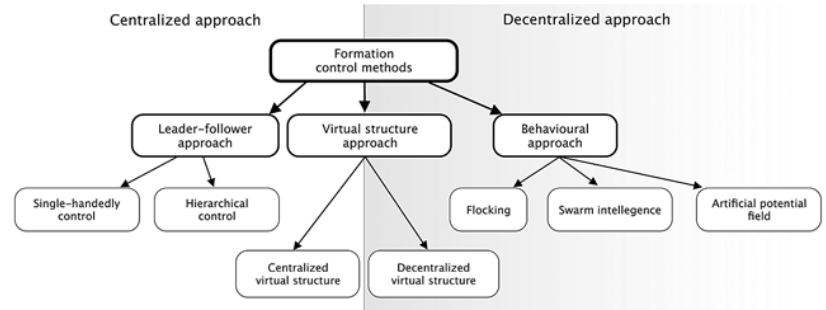
\includegraphics[width=\textwidth]{figures/klasifikasi_metode_kontrol_formasi.png}
    \caption{Klasifikasi metode untuk kontrol formasi \cite{kurochkinMethodsFormationControl2021}}
    \label{fig:klasifikasi-metode-kontrol-formasi}
\end{figure}

\textit{Leader-follower} mengandalkan satu agen sebagai pemimpin yang menentukan lintasan, sementara agen lainnya mengikuti dengan menjaga jarak atau posisi relatif tertentu. Pendekatan ini sederhana dan stabil, namun memiliki kelemahan berupa ketergantungan tinggi pada \textit{leader}, sehingga jika \textit{leader} gagal atau terhambat, formasi bisa terganggu secara keseluruhan \cite{abroComprehensiveReviewNextGen2025}. \textit{Virtual structure} memperlakukan semua agen sebagai bagian dari satu kesatuan struktur kaku, memberikan kestabilan formasi yang tinggi. Namun, pendekatan ini kurang fleksibel terhadap perubahan lingkungan dan sulit diterapkan pada skenario dinamis yang memerlukan adaptasi formasi \cite{renFormationFeedbackControl2004, liuDecentralizationVirtualLinkage2018}. Sementara itu, \textit{behavior-based} mengandalkan aturan lokal seperti penghindaran tabrakan dan penjagaan jarak untuk menghasilkan perilaku kolektif secara desentralisasi. Pendekatan ini adaptif dan responsif, namun memiliki kelemahan berupa potensi konflik antar aturan serta membutuhkan penyetelan parameter yang cermat agar sistem dapat berperilaku stabil dan terkoordinasi \cite{balchBehaviorbasedFormationControl1998}.

Kombinasi pendekatan \textit{virtual structure}, \textit{behavior-based}, dan \textit{leader-follower} banyak digunakan dalam sistem formasi yang memerlukan stabilitas, fleksibilitas, dan kemampuan adaptasi terhadap lingkungan dinamis. Oleh karena itu, penelitian tesis ini mengadopsi ketiga pendekatan tersebut: \textit{virtual structure} digunakan sebagai kerangka formasi, \textit{behavior-based} untuk penghindaran rintangan dan interaksi agen, dan \textit{leader-follower} untuk skenario jalur sempit atau kompleks.

Selain itu, pendekatan pengontrolan formasi juga dapat diklasifikasikan berdasarkan cara representasi formasi, yaitu \textit{position-based}, \textit{displacement-based}, dan \textit{distance-based} \cite{ohSurveyMultiagentFormation2015}. \textit{Position-based} membutuhkan posisi absolut setiap agen, sehingga bergantung pada GPS (\textit{Global Positioning System}) dan rentan terhadap gangguan sinyal \cite{ohSurveyMultiagentFormation2015}. \textit{Displacement-based} menggunakan pergeseran relatif antar agen, namun rentan terhadap akumulasi \textit{error} \cite{ohSurveyMultiagentFormation2015}. \textit{Distance-based} hanya menjaga jarak antar agen sesuai target tanpa arah eksplisit, sehingga lebih tangguh terhadap gangguan eksternal dan cocok untuk sistem desentralisasi \cite{ohSurveyMultiagentFormation2015}.

\begin{figure}[h]
    \centering
    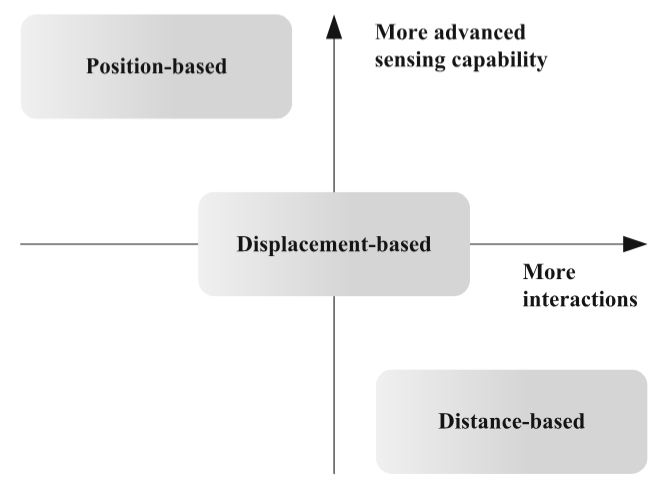
\includegraphics[width=0.75\textwidth]{figures/klasifikasi_representasi_formasi.png}
    \caption{Klasifikasi representasi formasi \cite{ohSurveyMultiagentFormation2015}}
    \label{fig:klasifikasi-representasi-formasi}
\end{figure}

Metode penghindaran rintangan yang digunakan adalah \textit{Artificial Potential Field} (APF), yang menghasilkan gaya tarik menuju tujuan dan gaya tolak dari rintangan \cite{wangUAVFormationObstacle2021}. Untuk mengatasi kelemahan APF yang rentan terhadap minimum lokal, digunakan pendekatan \textit{Improved Artificial Potential Field} (IAPF) yang menambahkan gaya random dan kontrol formasi \cite{wangUAVFormationObstacle2021, buiEventbasedReconfigurationControl2025}. Selanjutnya, digunakan juga pendekatan \textit{Event-Based Reconfiguration Control} (ERC) yang membuat formasi berubah secara dinamis sesuai kondisi lingkungan \cite{buiEventbasedReconfigurationControl2025}. Pendekatan ERC ini digunakan dalam perencanaan lintasan dan diintegrasikan ke dalam simulasi model non-linear quadcopter \cite{brescianiniNonlinearQuadrocopterAttitude2013a}, dengan penurunan dinamika menggunakan metode Kane \cite{johnBobzwikQuadcopter_SimCon2025, kaneDynamicsTheoryApplications1985}.

Pada penelitian oleh Quan \textit{et al.} \cite{quanDistributedSwarmTrajectory2022b, quanRobustEfficientTrajectory2023} telah berhasil mengimplementasikan metode optimisasi lintasan terdistribusi pada sistem wahana otonom nyata untuk terbang formasi di lingkungan yang padat rintangan. Penelitian tersebut mendemonstrasikan bahwa sistem desentralisasi dapat bekerja secara efisien dan kokoh (\textit{robust}) di dunia nyata jika dirancang untuk menangani kendala perangkat keras. Sejalan dengan arah perkembangan literatur tersebut, penelitian tesis ini akan membawa arsitektur kontrol ERC yang sebelumnya dikembangkan di lingkungan simulasi menuju realisasi \textit{hardware}. Implementasi fisik ini diusulkan untuk memvalidasi secara empiris efisiensi komunikasi dan keandalan mekanisme rekonfigurasi ERC saat dihadapkan langsung pada dinamika penerbangan nyata, latensi jaringan, dan derau sensor.

Penelitian tesis ini akan merujuk pada beberapa penelitian utama sebagai dasar pengembangan model, algoritma, dan rancangan implementasi perangkat keras. Rujukan utama yang digunakan dirangkum pada Tabel~\ref{tab:studi-terkait-rujukan}.

\begin{table}[h]
    \centering
    \caption{Studi terkait yang digunakan sebagai bahan rujukan}
    \label{tab:studi-terkait-rujukan}
    \small
    \begin{tabularx}{\textwidth}{|>{\centering\arraybackslash}p{1.3cm}|X|p{3.2cm}|X|}
        \hline
        \rowcolor{gray!20}
        \thead{Tahun} & \thead{Judul Penelitian/\\Proyek} & \thead{Penulis/\\Author} & \thead{Keterangan} \\
        \hline
        2023 & \textit{Quadcopter Simulation and Control. Dynamics generated with PyDy} \cite{johnBobzwikQuadcopter_SimCon2025} & John Bass & Referensi penurunan \textit{state-space} quadcopter. \\
        \hline
        2025 & \textit{Event-based Reconfiguration Control for Time-varying Formation of Robot Swarms in Narrow Spaces} \cite{buiEventbasedReconfigurationControl2025} & Duy-Nam Bui, Manh Duong Phung, dan Hung Pham Duy & Referensi penggunaan ERC. \\
        \hline
        2022 & \textit{Distributed Swarm Trajectory Optimization for Formation Flight in Dense Environments} \cite{quanDistributedSwarmTrajectory2022b} & Lun Quan, Longji Yin, Chao Xu, dan Fei Gao & Referensi implementasi \textit{hardware}. \\
        \hline
        2023 & \textit{Robust and Efficient Trajectory Planning for Formation Flight in Dense Environments} \cite{quanRobustEfficientTrajectory2023} & Lun Quan, Longji Yin, Tingrui Zhang, Mingyang Wang, Ruilin Wang, Sheng Zhong, Xin Zhou, Yanjun Cao, Chao Xu, dan Fei Gao & Referensi perencanaan lintasan formasi pada lingkungan padat rintangan. \\
        \hline
    \end{tabularx}
\end{table}

\section{Quadcopter}
Quadcopter, dengan empat motornya, merupakan sistem mekatronika dari konsep robot terbang \textit{Unmanned Aerial Vehicle} (UAV) dengan interaksi antara gaya aerodinamika, dinamika rotasi motor, dan gerakan bodi tegar secara keseluruhan untuk menentukan perilaku terbangnya. Motor diletakkan pada sudut-sudut dari quadcopter yang dapat dilihat seperti pada Gambar~\ref{fig:quadcopter-speedybee35}.

\begin{figure}[h]
    \centering
    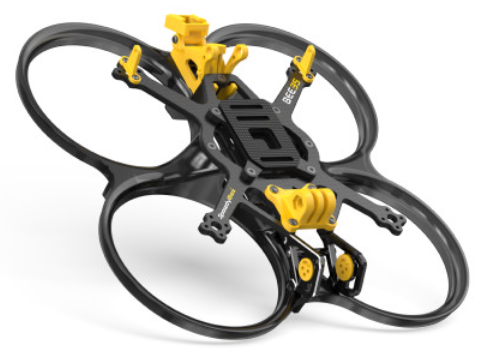
\includegraphics[width=0.5\textwidth]{figures/quadcopter_speedybee35.png}
    \caption{Quadcopter dengan kerangka SpeedyBee35 \cite{SpeedyBeeBee3535a}}
    \label{fig:quadcopter-speedybee35}
\end{figure}

Terdapat dua konfigurasi pemasangan motor yang umum digunakan pada quadcopter, yaitu konfigurasi ``+'' (\textit{plus}) dan konfigurasi ``X'' (\textit{cross}). Pada konfigurasi ``+'', lengan quadcopter sejajar dengan sumbu longitudinal dan lateral wahana, sehingga satu motor berada pada arah depan, satu motor pada arah belakang, dan dua motor lainnya berada pada sisi kanan serta kiri. Sementara itu, pada konfigurasi ``X'', lengan quadcopter membentuk sudut sekitar $45^{\circ}$ terhadap sumbu longitudinal dan lateral. Konfigurasi ``X'' banyak digunakan karena arah depan wahana berada di antara dua lengan, sehingga area pemasangan sensor atau kamera pada bagian depan relatif lebih terbuka. Ilustrasi perbedaan kedua konfigurasi tersebut ditunjukkan pada Gambar~\ref{fig:konfigurasi-quadcopter-plus-x}.

\begin{figure}[h]
    \centering
    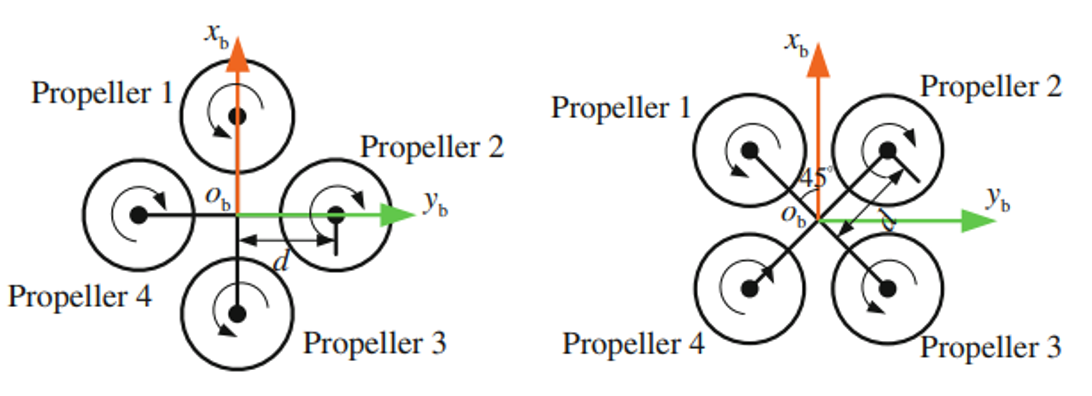
\includegraphics[width=0.85\textwidth]{figures/konfigurasi_quadcopter_plus_x.png}
    \caption{Konfigurasi pemasangan motor quadcopter: kiri ``+'' dan kanan ``X'' \cite{quanDynamicModelingExperiment2020}}
    \label{fig:konfigurasi-quadcopter-plus-x}
\end{figure}

Pengontrolan quadcopter dicapai dengan memanipulasi kecepatan putar keempat motor. Gerakan vertikal atau perubahan ketinggian dihasilkan dengan menaikkan atau menurunkan kecepatan seluruh motor secara bersamaan sehingga resultan gaya dorong total berubah. Sebaliknya, gerakan rotasi seperti \textit{roll}, \textit{pitch}, dan \textit{yaw} diperoleh dengan memberikan perbedaan kecepatan antar motor. Perbedaan gaya dorong pada sisi kanan dan kiri menghasilkan momen \textit{roll}, perbedaan gaya dorong pada sisi depan dan belakang menghasilkan momen \textit{pitch}, sedangkan perbedaan torsi reaksi antara pasangan motor yang berputar searah dan berlawanan arah jarum jam menghasilkan momen \textit{yaw}. Dengan demikian, perubahan posisi dan orientasi quadcopter merupakan hasil kombinasi dari gaya dorong total dan momen diferensial yang diberikan oleh aktuator motor.

Dalam pemodelan dinamika quadcopter, digunakan dua kerangka acuan utama, yaitu kerangka acuan inersia dan kerangka acuan bodi. Kerangka acuan inersia $N$ dianggap tetap terhadap permukaan bumi dan digunakan sebagai referensi absolut untuk menyatakan posisi serta orientasi wahana. Konvensi yang umum digunakan adalah NED (\textit{North-East-Down}), dengan sumbu $x_N$ mengarah ke utara, sumbu $y_N$ mengarah ke timur, dan sumbu $z_N$ mengarah ke bawah. Pada konvensi ini, percepatan gravitasi bernilai positif pada arah sumbu $z_N$.

Kerangka acuan bodi $B$ melekat kaku pada quadcopter dengan titik asal umumnya ditempatkan pada pusat massa (\textit{Center of Mass}/CoM). Sumbu-sumbu pada kerangka bodi dipilih mengikuti geometri utama wahana sehingga besaran seperti kecepatan linear bodi, kecepatan sudut, gaya dorong motor, dan torsi aktuator dapat dinyatakan secara lebih langsung. Dalam penelitian ini, kerangka bodi menggunakan konvensi FRD (\textit{Front-Right-Down}), yaitu sumbu $x_B$ mengarah ke depan quadcopter, sumbu $y_B$ mengarah ke kanan, dan sumbu $z_B$ mengarah ke bawah. Hubungan antara kerangka inersia NED dan kerangka bodi FRD ditunjukkan pada Gambar~\ref{fig:kerangka-acuan-ned-frd}.

\begin{figure}[h]
    \centering
    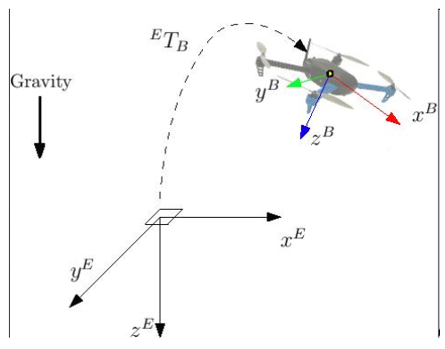
\includegraphics{figures/kerangka_acuan_ned_frd.png}
    \caption{Kerangka acuan inersia NED dan kerangka bodi FRD pada quadcopter \cite{quanDynamicModelingExperiment2020}}
    \label{fig:kerangka-acuan-ned-frd}
\end{figure}

\subsection{Model Dinamika Sistem Quadcopter}
Model dinamika quadcopter pada penelitian ini dirumuskan dalam kerangka inersia NED dan kerangka bodi FRD. Penurunan persamaan gerak dilakukan menggunakan Metode Kane karena metode ini dapat menyusun dinamika benda tegar secara sistematis melalui koordinat umum, kecepatan umum, serta daftar gaya dan torsi yang bekerja pada sistem \cite{kaneDynamicsTheoryApplications1985}. Keadaan sistem dinyatakan oleh posisi pusat massa, orientasi, kecepatan translasi, dan kecepatan sudut bodi. Orientasi direpresentasikan menggunakan quaternion untuk menghindari singularitas yang umum muncul pada representasi sudut Euler. Dengan demikian, vektor keadaan plant yang digunakan ditunjukkan pada Persamaan~\ref{eq:state-plant-quadcopter}.
\begin{equation}
    \mathbf{s}_{\mathrm{plant}} =
    \begin{bmatrix}
        x & y & z & q_w & q_x & q_y & q_z & \dot{x} & \dot{y} & \dot{z} & p & q & r
    \end{bmatrix}^{T},
    \label{eq:state-plant-quadcopter}
\end{equation}
di mana $(x,y,z)$ adalah posisi pusat massa pada kerangka $N$, $(q_w,q_x,q_y,q_z)$ adalah quaternion orientasi bodi terhadap kerangka inersia, sedangkan $(p,q,r)$ adalah kecepatan sudut bodi terhadap sumbu $x_B$, $y_B$, dan $z_B$.

Kinematika translasi diperoleh dari turunan posisi pusat massa, sedangkan kinematika rotasi dinyatakan melalui hubungan antara turunan quaternion dan kecepatan sudut bodi. Hubungan kinematika quaternion tersebut diringkas pada Persamaan~\ref{eq:quaternion-kinematics}.
\begin{equation}
    \dot{\mathbf{q}} = \frac{1}{2}\mathbf{Q}(\mathbf{q})
    \begin{bmatrix}
        p & q & r
    \end{bmatrix}^{T},
    \label{eq:quaternion-kinematics}
\end{equation}
dengan $\mathbf{q}=[q_w\ q_x\ q_y\ q_z]^T$ dan $\mathbf{Q}(\mathbf{q})$ merupakan matriks transformasi quaternion. Selama simulasi, quaternion dinormalisasi agar memenuhi kendala $q_w^2+q_x^2+q_y^2+q_z^2=1$.

Dinamika translasi quadcopter ditentukan oleh gaya gravitasi, gaya dorong total motor, dan gaya hambat aerodinamis. Bentuk ringkas persamaan gaya translasi ditunjukkan pada Persamaan~\ref{eq:translational-dynamics}.
\begin{equation}
    m\ddot{\mathbf{p}} = \mathbf{F}_g + \mathbf{R}_{B}^{N}\mathbf{F}_T + \mathbf{F}_{\mathrm{drag}},
    \label{eq:translational-dynamics}
\end{equation}
Pada Persamaan~\ref{eq:translational-dynamics}, $m$ adalah massa quadcopter, $\mathbf{R}_{B}^{N}$ adalah matriks rotasi dari kerangka bodi ke kerangka inersia, dan $\mathbf{F}_T$ adalah resultan gaya dorong motor pada kerangka bodi. Untuk konvensi FRD, gaya dorong motor bekerja berlawanan arah dengan sumbu $z_B$, sehingga resultan gaya dorong total dinyatakan pada Persamaan~\ref{eq:total-thrust}.
\begin{equation}
    \mathbf{F}_T =
    \begin{bmatrix}
        0 & 0 & -(T_1+T_2+T_3+T_4)
    \end{bmatrix}^{T}.
    \label{eq:total-thrust}
\end{equation}

Dinamika rotasi diperoleh dari keseimbangan momen pada bodi quadcopter. Dengan tensor inersia $\mathbf{I}=\mathrm{diag}(I_{xx},I_{yy},I_{zz})$, bentuk ringkas persamaan rotasi ditunjukkan pada Persamaan~\ref{eq:rotational-dynamics}.
\begin{equation}
    \mathbf{I}\dot{\boldsymbol{\omega}} + \boldsymbol{\omega}\times(\mathbf{I}\boldsymbol{\omega})
    = \boldsymbol{\tau}_{T} + \boldsymbol{\tau}_{M} + \boldsymbol{\tau}_{\mathrm{gyro}},
    \label{eq:rotational-dynamics}
\end{equation}
Pada Persamaan~\ref{eq:rotational-dynamics}, $\boldsymbol{\omega}=[p\ q\ r]^T$, $\boldsymbol{\tau}_{T}$ adalah momen akibat perbedaan gaya dorong antar motor, $\boldsymbol{\tau}_{M}$ adalah torsi reaktif motor, dan $\boldsymbol{\tau}_{\mathrm{gyro}}$ adalah torsi giroskopik rotor. Untuk konfigurasi ``X'', kombinasi perbedaan gaya dorong motor menghasilkan momen \textit{roll} dan \textit{pitch}, sedangkan perbedaan torsi reaktif pasangan motor menghasilkan momen \textit{yaw}.

Gaya dorong dan torsi reaktif masing-masing motor dimodelkan sebagai fungsi kuadrat dari kecepatan sudut motor, seperti ditunjukkan pada Persamaan~\ref{eq:motor-thrust-torque}.
\begin{equation}
    T_i = k_T\omega_i^2, \qquad \tau_i = k_Q\omega_i^2,
    \label{eq:motor-thrust-torque}
\end{equation}
dengan $k_T$ sebagai koefisien gaya dorong dan $k_Q$ sebagai koefisien torsi. 

Respons aktuator motor tidak dianggap instan, tetapi dimodelkan sebagai sistem dinamis sederhana agar simulasi lebih mendekati perilaku motor fisik. Secara umum, hubungan antara sinyal perintah kontrol yang dikirim ke motor, $u_{Mi}$, dan kecepatan angular aktual yang dihasilkan, $\omega_{Mi}$, dimodelkan sebagai sebuah sistem linear orde kedua. 

Pendekatan ini merepresentasikan adanya jeda waktu dan karakteristik respons dari motor fisik. Persamaan diferensial yang mengatur percepatan angular motor ($\ddot{\omega}_{Mi}$) ditunjukkan pada Persamaan~\ref{eq:dinamika_motor}.

\begin{equation}
    \ddot{\omega}_{Mi} = \frac{-2 \zeta \xi \dot{\omega}_{Mi} - \omega_{Mi} + k_p u_{Mi}}{\xi^2}
    \label{eq:dinamika_motor}
\end{equation}

di mana $k_p$ adalah \textit{gain} statis motor, $\xi$ adalah konstanta waktu sistem yang berhubungan dengan seberapa cepat motor merespons, dan $\zeta$ adalah rasio redaman (\textit{damping ratio}) yang menentukan apakah respons motor akan berosilasi atau mulus.

Secara keseluruhan, model \textit{plant} quadcopter (dengan 13 \textit{state} kinematika dan dinamika bodi) serta model aktuator motor (dengan 8 \textit{state} dinamika putaran motor) digabungkan membentuk sebuah sistem persamaan diferensial non-linear dengan total 21 \textit{state}. Persamaan \textit{state-space} dari sistem terintegrasi penuh ditunjukkan pada Persamaan~\ref{eq:state_space_21}.

\begin{equation}
\resizebox{0.95\textwidth}{!}{$
\dot{\mathbf{s}}(t) = \frac{d}{dt}
\begin{bmatrix}
x \\ y \\ z \\ q_w \\ q_x \\ q_y \\ q_z \\ \dot{x} \\ \dot{y} \\ \dot{z} \\ \omega_\phi \\ \omega_\theta \\ \omega_\psi \\ \omega_{M1} \\ \dot{\omega}_{M1} \\ \omega_{M2} \\ \dot{\omega}_{M2} \\ \omega_{M3} \\ \dot{\omega}_{M3} \\ \omega_{M4} \\ \dot{\omega}_{M4}
\end{bmatrix}
=
\begin{bmatrix}
\dot{x} \\
\dot{y} \\
\dot{z} \\
-0.5(\omega_\phi q_x + \omega_\theta q_y + \omega_\psi q_z) \\
0.5(\omega_\phi q_w - \omega_\theta q_z + \omega_\psi q_y) \\
0.5(\omega_\phi q_z + \omega_\theta q_w - \omega_\psi q_x) \\
-0.5(\omega_\phi q_y - \omega_\theta q_x - \omega_\psi q_w) \\
\frac{C_d \text{sign}(v_w \cos q_{w1} \cos q_{w2} - \dot{x})(v_w \cos q_{w1} \cos q_{w2} - \dot{x})^2 - 2(q_w q_y + q_x q_z)(T_{M1} + T_{M2} + T_{M3} + T_{M4})}{m_B} \\
\frac{C_d \text{sign}(v_w \sin q_{w1} \cos q_{w2} - \dot{y})(v_w \sin q_{w1} \cos q_{w2} - \dot{y})^2 + 2(q_w q_x - q_y q_z)(T_{M1} + T_{M2} + T_{M3} + T_{M4})}{m_B} \\
\frac{-C_d \text{sign}(v_w \sin q_{w2} + \dot{z})(v_w \sin q_{w2} + \dot{z})^2 - (T_{M1} + T_{M2} + T_{M3} + T_{M4})(q_w^2 - q_x^2 - q_y^2 + q_z^2) + g m_B}{m_B} \\
\frac{(I_{Byy} - I_{Bzz})\omega_\theta \omega_\psi - u_p I_{Rzz}(\omega_{M1} - \omega_{M2} + \omega_{M3} - \omega_{M4})\omega_\theta + (T_{M1} - T_{M2} - T_{M3} + T_{M4})d_{ym}}{I_{Bxx}} \\
\frac{(I_{Bzz} - I_{Bxx})\omega_\phi \omega_\psi + u_p I_{Rzz}(\omega_{M1} - \omega_{M2} + \omega_{M3} - \omega_{M4})\omega_\phi + (T_{M1} + T_{M2} - T_{M3} - T_{M4})d_{xm}}{I_{Byy}} \\
\frac{(I_{Bxx} - I_{Byy})\omega_\phi \omega_\theta + \tau_{M1} - \tau_{M2} + \tau_{M3} - \tau_{M4}}{I_{Bzz}} \\
\dot{\omega}_{M1} \\
\frac{-2 \zeta \xi \dot{\omega}_{M1} - \omega_{M1} + k_p u_{M1}}{\xi^2} \\
\dot{\omega}_{M2} \\
\frac{-2 \zeta \xi \dot{\omega}_{M2} - \omega_{M2} + k_p u_{M2}}{\xi^2} \\
\dot{\omega}_{M3} \\
\frac{-2 \zeta \xi \dot{\omega}_{M3} - \omega_{M3} + k_p u_{M3}}{\xi^2} \\
\dot{\omega}_{M4} \\
\frac{-2 \zeta \xi \dot{\omega}_{M4} - \omega_{M4} + k_p u_{M4}}{\xi^2}
\end{bmatrix}
$}
\label{eq:state_space_21}
\end{equation}

Berdasarkan Persamaan~\ref{eq:state_space_21}, sistem ini digunakan sebagai dasar simulasi respons quadcopter terhadap perintah kontrol, gangguan angin, serta perubahan konfigurasi formasi. Penyelesaian numeriknya dilakukan menggunakan integrator Runge--Kutta adaptif sehingga dinamika cepat pada aktuator dan dinamika gerak bodi dapat dihitung secara stabil dan efisien.


\subsection{Arsitektur Fisik dan Komponen Elektronik Quadcopter}
Wahana eksperimental yang digunakan dalam penelitian ini adalah quadcopter dengan konfigurasi tipe `X'. Pengembangan platform perangkat keras ini merupakan kelanjutan langsung dari arsitektur fisik platform pada penelitian sebelumnya \cite{argilianaPengembanganSistemKontrol2025}, yang kemudian ditingkatkan untuk mendukung komputasi desentralisasi penuh secara \textit{on-board}.

Secara umum, arsitektur fisik quadcopter terdiri dari struktur mekanik, sistem propulsi, sistem kontrol terbang, sistem komputasi tingkat tinggi, subsistem daya, serta jalur komunikasi antarkomponen. Platform quadcopter SpeedyBee 35 digunakan sebagai acuan arsitektur perangkat keras pada bagian ini. Wahana eksperimental ini menggunakan konfigurasi tipe `X' dan merupakan kelanjutan langsung dari arsitektur fisik platform pada penelitian sebelumnya \cite{argilianaPengembanganSistemKontrol2025}, yang kemudian ditingkatkan untuk mendukung komputasi kontrol desentralisasi secara penuh di atas wahana (\textit{on-board}).

Berikut adalah penjelasan rincian komponen perangkat keras yang diintegrasikan pada wahana:

\subsubsection{1. Platform Utama (SpeedyBee 35)}
Sebagai acuan dasar geometri dan dimensi mekanis, wahana ini menggunakan basis \textit{frame} quadcopter SpeedyBee 35. Desain kerangka yang kompak ini dipilih agar ideal untuk pergerakan navigasi di dalam ruangan (\textit{indoor}) namun tetap kuat menopang komponen avionik tambahan. Wujud platform acuan ini ditunjukkan pada Gambar~\ref{fig:quadcopter-speedybee35}.

\subsubsection{2. Struktur Fisik dan Komponen (Tampak Atas-Bawah)}
Untuk menyiasati keterbatasan ruang pada \textit{frame}, komponen elektronik dibagi menjadi dua area penempatan utama, yaitu pada sisi atas dan sisi bawah kerangka. Komponen tingkat tinggi seperti \textit{companion computer} dan modul komunikasi nirkabel diletakkan pada bagian atas wahana untuk mengoptimalkan ruang kerja sensor serta memudahkan akses antarmuka data. Sementara itu, komponen sistem propulsi dan kontrol dasar seperti \textit{flight controller}\label{abbr:fc} serta \textit{Electronic Speed Controller} (ESC) ditempatkan di bagian bawah atau inti kerangka. Susunan vertikal (\textit{stacking}) yang memisahkan komponen manajemen data dan manajemen daya ini diatur sedemikian rupa guna menjaga keseimbangan pusat massa (\textit{center of mass}) wahana tetap berada di tengah, seperti diperlihatkan pada Gambar~\ref{fig:struktur_fisik}.

\begin{figure}[h]
    \centering
    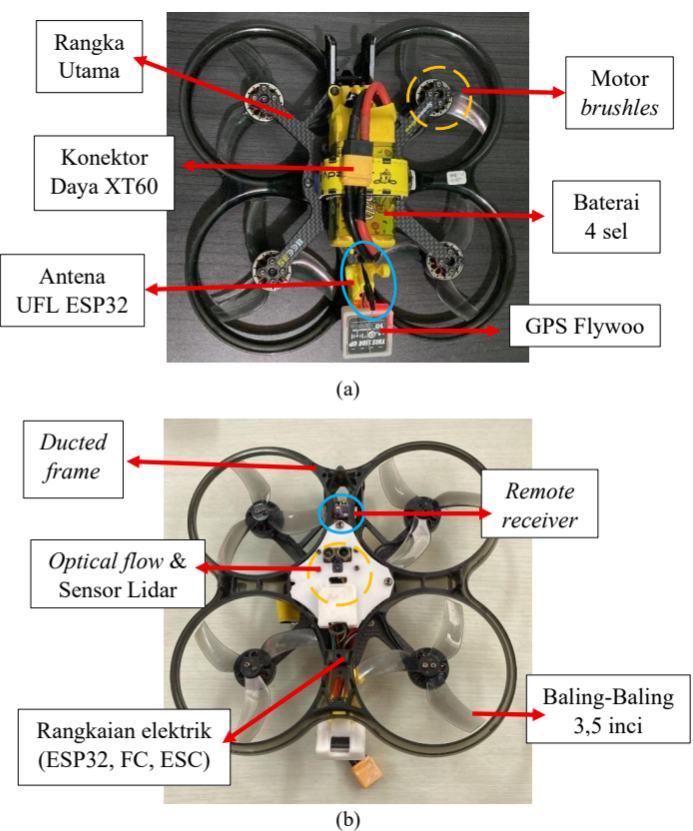
\includegraphics[width=0.55\textwidth]{figures/struktur_fisik.png}
    \caption{Struktur Fisik dan Tata Letak Komponen (a) Tampak Atas dan (b) Tampak Bawah \cite{argilianaPengembanganSistemKontrol2025}}
    \label{fig:struktur_fisik}
\end{figure}

\subsubsection{3. Sistem Elektronik Inti (ESC-FC)}
Stabilisasi tingkat rendah (\textit{inner-loop control}) dikoordinasikan secara penuh oleh integrasi \textit{Flight Controller} (FC) dan \textit{Electronic Speed Controller} (ESC) yang disusun terpadu dalam satu kesatuan struktur vertikal (\textit{stack topology}). \textit{Flight controller} berada di sisi atas sebagai unit pemroses mikro yang dilengkapi sensor \textit{Inertial Measurement Unit} (IMU) untuk mengestimasi orientasi sikap wahana secara \textit{real-time}. Modul FC ini terhubung ke papan 4-in-1 ESC di bawahnya melalui \textit{interconnect cable harness} untuk mentransmisikan sinyal komando kecepatan motor. ESC kemudian bertugas menerjemahkan sinyal kontrol tersebut menjadi regulasi arus multi-fasa guna menggerakkan keempat motor BLDC secara sinkron. Guna menjaga akurasi pembacaan sensor IMU dari derau mekanis yang dihasilkan oleh putaran motor, seluruh struktur \textit{stack} ini dipasang memanfaatkan karet peredam (\textit{anti-vibration damping silicone grommets}), seperti diperlihatkan pada Gambar~\ref{fig:esc_fc}.

\begin{figure}[h]
    \centering
    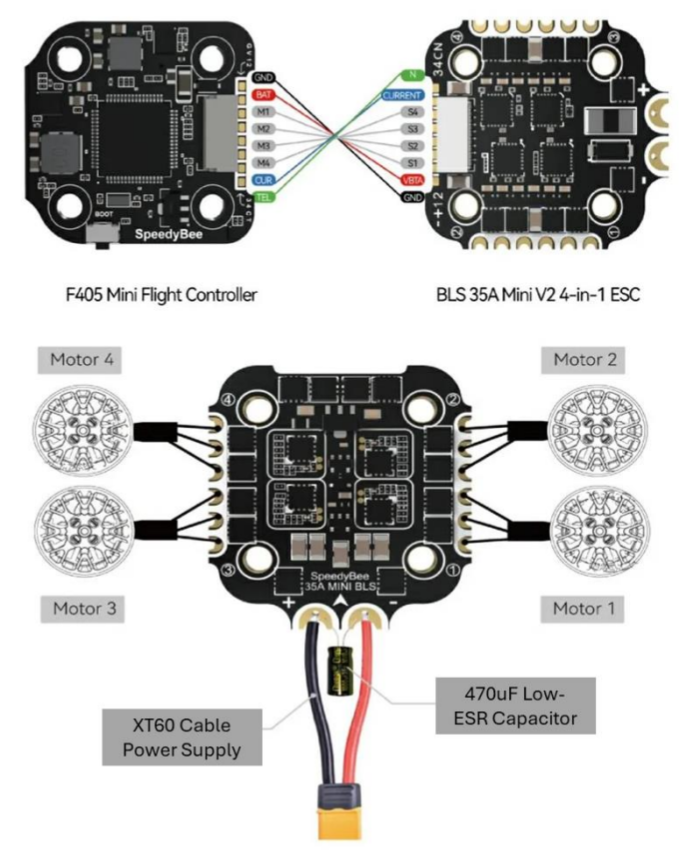
\includegraphics[width=0.45\textwidth]{figures/esc_fc.png}
    \caption{Integrasi Unit \textit{Electronic Speed Controller} (ESC) dan \textit{Flight Controller} (FC)}
    \label{fig:esc_fc}
\end{figure}

\subsubsection{4. Skematik Elektrik dan Pengabelan}
Sistem pengabelan (\textit{wiring}) pada wahana ini merangkum interkoneksi jalur distribusi daya dan alur komunikasi data antar subsistem elektronik. Sumber daya utama dari baterai LiPo dihubungkan secara langsung menuju papan \textit{Electronic Speed Controller} (ESC) 4-in-1 guna melayani kebutuhan arus tinggi bagi keempat motor \textit{brushless}. ESC tersebut kemudian mendistribusikan daya teregulasi (\textit{Battery Eliminator Circuit} / BEC) untuk menyalakan modul \textit{Flight Controller} (FC) SpeedyBee F405. 

Pada lapis komputasi tingkat tinggi, \textit{companion computer} (ESP-32) dihubungkan dengan FC melalui antarmuka serial UART (pin TX dan RX silang) guna memfasilitasi pertukaran pesan kontrol berbasis MAVLink secara \textit{real-time}. Selain itu, skematik ini juga memperlihatkan pemetaan sinyal kontrol motor dari FC ke ESC, serta koneksi \textit{receiver} radio (seperti TBS Crossfire) untuk keperluan kontrol \textit{override} manual atau intervensi \textit{fail-safe}. Skematik elektrik diagram pengabelan (\textit{wiring diagram}) ini ditunjukkan secara menyeluruh pada Gambar~\ref{fig:wiring_diagram}.

\begin{figure}[h]
    \centering
    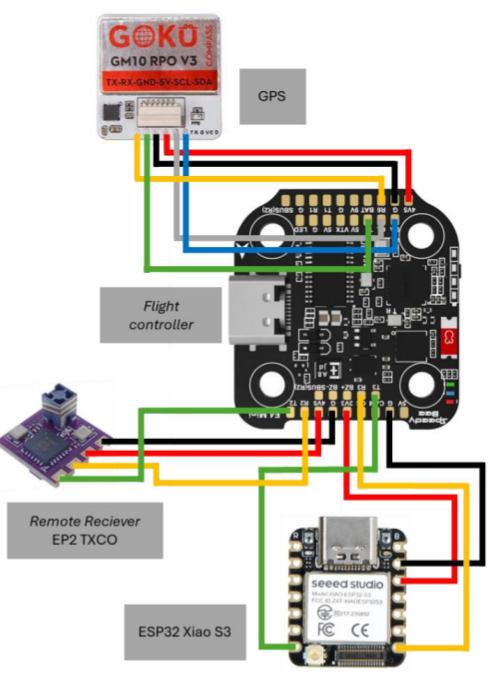
\includegraphics[width=0.35\textwidth]{figures/wiring_diagram.png}
    \caption{Skematik Elektrik dan Diagram Pengabelan Seluruh Komponen Wahana}
    \label{fig:wiring_diagram}
\end{figure}

\subsection{Protokol Komunikasi}
Sistem komunikasi kawanan quadcopter dirancang dengan memisahkan secara jelas antara lapisan protokol data (\textit{software}) dan arsitektur jaringan fisik (\textit{hardware}). Baik komunikasi antar-wahana (Quadcopter-Quadcopter) maupun komunikasi stasiun darat (Quadcopter-GCS) secara seragam mengadopsi protokol pesan biner \textbf{MAVLink} (\textit{Micro Air Vehicle Link}) yang ditransmisikan di atas media jaringan \textbf{Wi-Fi lokal} berbasis soket UDP (\textit{User Datagram Protocol}) \cite{chenReviewUnmannedAerial2020, linLeaderFollowerUAV2026}. Perbedaan utama dari kedua jalur komunikasi ini terletak pada rute aliran dan topologi jaringannya.

\subsubsection{1. Komunikasi Antar-Wahana (Quadcopter-Quadcopter)}
Jalur komunikasi antar-wahana merupakan fondasi dari arsitektur kontrol terdesentralisasi. Modul Wi-Fi internal pada mikrokontroler ESP32 di setiap wahana dikonfigurasi untuk saling bertukar data secara langsung (\textit{point-to-point}) menggunakan metode soket UDP \textit{broadcast} atau \textit{multicast} tanpa melalui \textit{router} perantara. Jalur fisik mandiri ini digunakan untuk menyiarkan paket biner MAVLink yang berisi data \textit{state} kinematika aktual (posisi 3D dan kecepatan). Karakteristik paket MAVLink yang sangat ringan memastikan algoritma \textit{Event-Based Reconfiguration Control} (ERC) dapat mengeksekusi adaptasi formasi dengan latensi minimal dan bebas dari risiko pemutusan akibat kegagalan titik tunggal (\textit{single point of failure}) pada jaringan pusat.

\subsubsection{2. Komunikasi Stasiun Darat (Quadcopter-GCS)}
Jalur komunikasi stasiun darat memfasilitasi pemantauan telemetri dan kontrol intervensi jarak jauh. Berbeda dengan jalur antar-wahana, arsitektur jaringan pada jalur ini bersifat terpusat (\textit{centralized}) dengan memanfaatkan sebuah \textit{router} nirkabel sebagai \textit{access point} utama di dalam area pengujian \textit{indoor}. Melalui medium ini, setiap ESP32 mengirimkan paket telemetri MAVLink berupa data kesehatan sistem (\textit{heartbeat}), estimasi orientasi sikap (\textit{attitude}), dan kapasitas baterai menuju \textit{Ground Control Station} (GCS). Sebaliknya, GCS menggunakan jalur Wi-Fi terpusat ini untuk mengirimkan komando tingkat tinggi seperti perintah \textit{arm/disarm}, perpindahan mode terbang, atau komando pendaratan darurat secara \textit{real-time}.

\section{Sistem Lokalisasi \textit{Indoor} Berbasis Kamera Atas (\textit{Ceiling Camera})}

Mengingat pengujian navigasi kawanan \textit{quadcopter} dilakukan di lingkungan dalam ruangan (\textit{indoor}), sistem tidak dapat mengandalkan \textit{Global Positioning System} (GPS) untuk mendapatkan informasi posisi spasial absolut.
Sebagai solusinya, arsitektur perangkat keras ini memanfaatkan sistem lokalisasi eksternal berbasis penglihatan komputer (\textit{computer vision}) menggunakan kamera atas (\textit{fixed overhead/ceiling camera}) yang dipadukan dengan penanda visual (\textit{visual fiducial marker}) pada wahana.
Metode ini dipilih karena mampu memberikan tingkat presisi pelacakan posisi absolut dalam skala sentimeter ($\pm 1\text{--}3\text{ cm}$), bebas dari akumulasi penyimpangan posisi (\textit{drift}) seiring waktu, serta tidak terpengaruh oleh interferensi gelombang nirkabel (\textit{multipath fading}) yang kerap terjadi pada sensor berbasis sinyal radio di ruangan tertutup.

Sistem lokalisasi kamera atas yang diimplementasikan terdiri dari tiga komponen utama:
\begin{enumerate}
    \item \textbf{Kamera Sudut Lebar (\textit{Wide-Angle Overhead Camera}).} Satu unit kamera dipasang pada posisi statis di langit-langit area pengujian dengan orientasi menghadap tegak lurus ke bawah (\textit{nadir}). Kamera ini berfungsi sebagai penentu kerangka acuan inersia global (\textit{global reference frame}) yang mencakup seluruh area navigasi kawanan wahana.
    \item \textbf{Penanda Visual (\textit{AprilTag / ArUco Marker})} Dipasang secara datar pada bagian atas bodi masing-masing \textit{quadcopter}. Setiap wahana menggunakan pola matriks biner dengan identitas (ID) unik (misalnya ID 0 hingga 4 untuk lima wahana), sehingga sistem persepsi dapat membedakan dan melacak setiap agen secara simultan.
    \item \textbf{Stasiun Pemroses Citra (\textit{Vision Processing Base Station}).} Komputer di darat yang menerima aliran bingkai citra (\textit{video stream}) dari kamera untuk mengeksekusi algoritma ekstraksi posisi 3D dan orientasi wahana secara \textit{real-time}.
\end{enumerate}

Proses penentuan posisi spasial 3D dan orientasi sikap wahana didasarkan pada model kamera jarum pentul (\textit{pinhole camera model}) dan penyelesaian masalah \textit{Perspective-n-Point} (PnP).
Dengan mengasumsikan matriks kalibrasi intrinsik kamera $\mathbf{K}$ telah diketahui melalui proses kalibrasi awal, hubungan antara koordinat piksel $(u, v)$ pada bidang citra dan koordinat spasial absolut $(x_w, y_w, z_w)$ pada kerangka acuan dunia dinyatakan sebagai:
\begin{equation}
    s 
    \begin{bmatrix}
        u \\ v \\ 1
    \end{bmatrix}
    = \mathbf{K} 
    \begin{bmatrix}
        \mathbf{R} & \mathbf{T}
    \end{bmatrix}
    \begin{bmatrix}
        x_w \\ y_w \\ z_w \\ 1
    \end{bmatrix}
    \label{eq:pinhole_pnp}
\end{equation}
di mana $s$ adalah faktor skala kedalaman, $\mathbf{R} \in \mathbb{R}^{3 \times 3}$ adalah matriks rotasi 3D yang menggambarkan orientasi sikap wahana (khususnya sudut \textit{yaw} $\psi$), $\mathbf{T} = [x, y, z]^T$ adalah vektor translasi posisi 3D absolut \textit{quadcopter} terhadap pusat optik kamera, dan $\mathbf{K}$ adalah matriks intrinsik kamera yang didefinisikan sebagai:
\begin{equation}
    \mathbf{K} = 
    \begin{bmatrix}
        f_x & 0 & c_x \\
        0 & f_y & c_y \\
        0 & 0 & 1
    \end{bmatrix}
\end{equation}
dengan $(f_x, f_y)$ merepresentasikan panjang fokus (\textit{focal length}) dalam satuan piksel dan $(c_x, c_y)$ adalah titik pusat optik (\textit{principal point}).

Menggunakan dimensi fisik \textit{marker} yang telah diketahui (misalnya $10 \times 10\text{ cm}$) dan empat titik sudut \textit{marker} yang terdeteksi pada citra, sistem menyelesaikan Persamaan~\ref{eq:pinhole_pnp} menggunakan algoritma numerik \textit{SolvePnP} berbasis optimasi Levenberg--Marquardt.
Keluaran dari algoritma ini berupa estimasi koordinat spasial absolut $(x, y, z)$ dan sudut \textit{yaw} ($\psi$) secara \textit{real-time} untuk setiap wahana.

Data posisi dan orientasi terhitung dari komputer darat dikemas ke dalam format pesan biner MAVLink dan disiarkan melalui jaringan nirkabel (soket UDP/Wi-Fi) menuju \textit{companion computer} (ESP32) di masing-masing \textit{quadcopter}.
Meskipun sistem lokalisasi berbasis kamera atas memberikan referensi posisi absolut yang sangat akurat dan bebas dari \textit{drift}, keluaran datanya memiliki laju pembaruan (\textit{update rate}) yang dibatasi oleh laju bingkai kamera (misalnya 60 FPS) serta memiliki jeda waktu pemrosesan citra (\textit{latency processing}).
Oleh karena itu, data posisi spasial dari kamera atas ini tidak langsung diumpankan ke kalang pengontrol tingkat rendah, melainkan difusikan terlebih dahulu dengan data sensor internal berkecepatan tinggi (\textit{Inertial Measurement Unit}/IMU) melalui modul \textit{Extended Kalman Filter} (EKF) untuk menghasilkan estimasi \textit{state} yang mulus dan stabil.

\section{Sistem Deteksi Rintangan Berbasis Sensor Ultrasonik}

Selain informasi posisi absolut, kemampuan kawanan quadcopter untuk bermanuver dan mengubah formasi secara adaptif sangat bergantung pada persepsi spasial terhadap lingkungan di sekitarnya. Untuk memfasilitasi algoritma penghindaran tabrakan (\textit{collision avoidance}) dan pemicu rekonfigurasi adaptif pada strategi \textit{Event-Based Reconfiguration Control} (ERC), wahana dilengkapi dengan sistem deteksi rintangan berbasis sensor ultrasonik \cite{siegwartIntroductionAutonomousMobile2004}.

Sensor ultrasonik dipilih karena kemampuannya memberikan pengukuran jarak linier yang akurat pada jarak dekat hingga menengah, serta beban komputasinya yang sangat ringan bagi mikrokontroler. Pada perancangan perangkat keras ini, sepasang sensor ultrasonik diposisikan secara strategis menghadap ke arah lateral, yaitu satu sensor di sisi kiri dan satu sensor di sisi kanan kerangka quadcopter. Penempatan lateral ini secara khusus ditujukan untuk mengukur jarak wahana terhadap dinding atau rintangan di sekitarnya saat melintasi lorong sempit.

Prinsip kerja sensor ultrasonik didasarkan pada pancaran gelombang suara frekuensi tinggi (umumnya 40 kHz) yang memantul kembali ketika mengenai permukaan sebuah objek padat. Jarak rintangan ($d_{\text{obs}}$) dihitung menggunakan prinsip waktu tempuh pantulan (\textit{Time of Flight}) gelombang suara dengan persamaan dasar \cite{borensteinObstacleAvoidanceUltrasonic1988}:
\begin{equation}
    d_{\text{obs}} = \frac{v_{\text{suara}} \cdot t_{\text{pantul}}}{2}
\end{equation}
di mana $v_{\text{suara}}$ adalah kecepatan rambat suara di udara (sekitar $343$ m/s pada suhu ruangan $20^\circ\text{C}$), dan $t_{\text{pantul}}$ adalah waktu tempuh bolak-balik terukur sejak gelombang dipancarkan hingga pantulannya (\textit{echo}) diterima kembali oleh \textit{receiver} pada sensor.

Dalam arsitektur sistem ini, hasil pembacaan jarak dari sensor kiri ($d_l$\label{sym:dl}) dan sensor kanan ($d_r$\label{sym:dr}) diakuisisi secara periodik oleh \textit{companion computer} (ESP32). Data dari kedua sensor ini kemudian dikalkulasi untuk menghasilkan estimasi ketersediaan lebar lingkungan aktual ($w_e$\label{sym:we}) tegak lurus terhadap arah gerak wahana. Formulasi matematis untuk estimasi lebar lorong ini dinyatakan sebagai:
\begin{equation}
    w_e = d_l + d_r + w_{\text{body}}
\end{equation}
di mana $w_{\text{body}}$\label{sym:wbody} merepresentasikan lebar fisik struktural dari bodi quadcopter itu sendiri (jarak ujung-ke-ujung antar sensor). 

Variabel $w_e$ ini berfungsi sebagai parameter utama yang diumpankan ke perencana tingkat tinggi. Jika total jarak bebas lateral menyempit dan nilai $w_e$ turun melewati ambang batas toleransi formasi ideal, sistem akan mengenali kondisi tersebut sebagai rintangan lorong sempit dan memicu transisi mode formasi menjadi \textit{tailgating} (mengekor). Skema pengukuran dan penempatan sensor ini dapat dilihat pada Gambar~\ref{fig:ultrasonic_placement}.


\begin{figure}[htbp]
    \centering
    \resizebox{0.85\textwidth}{!}{%
    \begin{tikzpicture}[
        >=Stealth,
        wall/.style={draw, thick, fill=gray!20},
        frame/.style={draw=blue!60!black, line width=3.5pt},
        hub/.style={draw=blue!60!black, thick, fill=blue!8, rounded corners=2pt},
        rotor/.style={draw=gray!80!black, thick, fill=gray!10, circle, minimum size=0.9cm, inner sep=0pt},
        sensor/.style={draw, thick, fill=black, minimum width=0.16cm, minimum height=0.4cm},
        beam/.style={fill=cyan!30, opacity=0.5},
        measure/.style={<->, thick},
        guide/.style={dotted, gray!70, thick},
        label/.style={font=\small, align=center}
    ]
        % Dinding kiri dan kanan
        \draw[wall] (-4.0,-2.5) rectangle (-3.75,4.0);
        \draw[wall] (3.75,-2.5) rectangle (4.0,4.0);
        \node[label, rotate=90] at (-4.45,0.5) {Dinding\\kiri};
        \node[label, rotate=-90] at (4.45,0.5) {Dinding\\kanan};

        % Lengan quadcopter (konfigurasi X)
        \draw[frame] (-0.8,0.8) -- (0.8,-0.8);
        \draw[frame] (-0.8,-0.8) -- (0.8,0.8);

        % Kerucut pancaran ultrasonik diperlebar.
        % Sensor kiri depan (pusat di -1.0, 1.0; arah 135 derajat)
        \begin{scope}[shift={(-1.0,1.0)}, rotate=100]
            \fill[beam] (0,0) -- (-40:3.8) arc (-40:40:3.8) -- cycle;
        \end{scope}
        % Sensor kanan depan (pusat di 1.0, 1.0; arah 45 derajat)
        \begin{scope}[shift={(1.0,1.0)}, rotate=80]
            \fill[beam] (0,0) -- (-40:3.8) arc (-40:40:3.8) -- cycle;
        \end{scope}

        % Rotor quadcopter
        \node[rotor] at (-0.8,0.8) {}; \filldraw[gray!80!black] (-0.8,0.8) circle (0.05); % Kiri Depan
        \node[rotor] at (0.8,0.8) {};  \filldraw[gray!80!black] (0.8,0.8) circle (0.05);  % Kanan Depan
        \node[rotor] at (-0.8,-0.8) {}; \filldraw[gray!80!black] (-0.8,-0.8) circle (0.05); % Kiri Belakang
        \node[rotor] at (0.8,-0.8) {};  \filldraw[gray!80!black] (0.8,-0.8) circle (0.05);  % Kanan Belakang

        % Bodi pusat
        \draw[hub] (-0.4,-0.4) rectangle (0.4,0.4);
        \node[label, font=\scriptsize\bfseries] at (0,0) {FC /\\ESP32};

        % Panah penunjuk arah depan
        \draw[->, ultra thick, red!70!black] (0, 0.45) -- (0, 1.8) node[above, font=\small\bfseries] {Depan (Arah Gerak)};

        % Sensor ultrasonik kiri dan kanan depan diputar 45 derajat ke luar.
        \node[sensor, rotate=-45] (SL) at (-1.0, 1.0) {};
        \node[sensor, rotate=45] (SR) at (1.0, 1.0) {};
        \node[label, font=\scriptsize] at (-1.7, 0.6) {Sensor\\kiri};
        \node[label, font=\scriptsize] at (1.7, 0.6) {Sensor\\kanan};

        % Garis ukur jarak proyeksi lateral
        \draw[measure, dashed] (-3.75,1.0) -- (-1.0,1.0) node[midway, below] {$d_l$};
        \draw[measure, dashed] (1.0,1.0) -- (3.75,1.0) node[midway, below] {$d_r$};

        % Penanda jarak pembacaan mentah (miring 45 derajat)
        \draw[<->, gray!90!black, dashed, line width=1pt] (-3.75, 3.75) -- (-1.1, 1.1) 
            node[midway, sloped, above, font=\scriptsize] {$d_{\mathrm{raw\_l}}$};
        \draw[<->, gray!90!black, dashed, line width=1pt] (3.75, 3.75) -- (1.1, 1.1) 
            node[midway, sloped, above, font=\scriptsize] {$d_{\mathrm{raw\_r}}$};

        % Sudut theta
        \draw[thick] (-1.0, 1.6) arc (90:135:0.6);
        \node[font=\scriptsize] at (-1.3, 1.75) {$\theta$};
        \draw[thick] (1.0, 1.6) arc (90:45:0.6);
        \node[font=\scriptsize] at (1.3, 1.75) {$\theta$};

        % Garis ukur lebar bodi (jarak lateral antar pusat sensor)
        \draw[measure] (-1.0,-1.6) -- (1.0,-1.6) node[midway, below] {$w_{\mathrm{body}}$};

        % Garis ukur lebar lingkungan total
        \draw[measure, blue!70!black, line width=1.1pt] (-3.75,4.3) -- (3.75,4.3)
            node[midway, above, label, text=blue!70!black]
            {$w_e = d_l + d_r + w_{\mathrm{body}}$};

        % Garis bantu proyeksi pengukuran
        \draw[guide] (-3.75,1.0) -- (-3.75,4.5);
        \draw[guide] (3.75,1.0) -- (3.75,4.5);
        \draw[guide] (-1.0,1.0) -- (-1.0,-1.8);
        \draw[guide] (1.0,1.0) -- (1.0,-1.8);
        \draw[guide] (-1.0,1.0) -- (-1.0,2.0); % Garis lurus ke atas untuk sudut theta kiri
        \draw[guide] (1.0,1.0) -- (1.0,2.0);   % Garis lurus ke atas untuk sudut theta kanan

    \end{tikzpicture}%
    }
    \caption{Skema estimasi ketersediaan lebar lingkungan ($w_e$) menggunakan sensor ultrasonik yang diorientasikan secara diagonal dengan sudut $\theta$. Jarak lateral ke dinding ($d_l$ dan $d_r$) diekstraksi melalui proyeksi trigonometri dari pembacaan jarak mentah ($d_{\mathrm{raw\_l}}$ dan $d_{\mathrm{raw\_r}}$).}
    \label{fig:ultrasonic_placement}
\end{figure}

Setelah seluruh sistem persepsi---baik lokalisasi spasial menggunakan UWB maupun persepsi rintangan menggunakan ultrasonik---berhasil memetakan kondisi eksternal, kerangka kontrol membutuhkan estimasi \textit{state} internal wahana yang bersih dari derau agar dapat mengeksekusi manuver dengan stabil. Oleh karena itu, data posisi dari UWB diproses lebih lanjut pada modul estimator \textit{state}.

\section{Estimator \textit{State} dengan \textit{Extended Kalman Filter} (EKF)}

Keberhasilan manuver yang dihasilkan oleh perencana tingkat tinggi dan keandalan stabilisasi oleh pengontrol tingkat rendah sangat bergantung pada akurasi informasi \textit{state} aktual dari wahana. Mengingat dinamika quadcopter bersifat non-linear dan sensor pengukuran selalu memiliki derau (\textit{noise}), sistem ini dilengkapi dengan algoritma \textit{Extended Kalman Filter} (EKF) sebagai estimator \textit{state} utama \cite{KalmanFilterGeneralizations2006}. 

EKF berfungsi melakukan fusi data (\textit{sensor fusion}) secara \textit{real-time}. Algoritma ini menggabungkan data dari sensor internal bawaan seperti \textit{Inertial Measurement Unit} (IMU) yang memiliki laju pembaruan (\textit{update rate}) tinggi namun rentan terhadap \textit{drift} seiring waktu, dengan data dari sistem lokalisasi \textit{indoor} eksternal (seperti UWB) yang memberikan referensi posisi absolut. 

Secara matematis, sistem non-linear dari quadcopter dapat direpresentasikan dalam model ruang-keadaan (\textit{state-space}) diskrit sebagai berikut \cite{welchIntroductionKalmanFilter2006}:
\begin{align}
    \mathbf{x}_k &= f(\mathbf{x}_{k-1}, \mathbf{u}_{k-1}) + \mathbf{w}_{k-1} \label{eq:ekf_system} \\
    \mathbf{z}_k &= h(\mathbf{x}_k) + \mathbf{v}_k \label{eq:ekf_measurement}
\end{align}
di mana $\mathbf{x}_k \in \mathbb{R}^n$ adalah vektor \textit{state} sistem pada langkah waktu $k$ (mencakup posisi 3D, kecepatan linear, dan \textit{quaternion} orientasi), $\mathbf{u}_{k-1} \in \mathbb{R}^m$ adalah vektor masukan kontrol, dan $\mathbf{z}_k \in \mathbb{R}^p$ adalah vektor pengukuran aktual dari sensor (seperti koordinat posisi spasial dari UWB). Variabel $\mathbf{w}_{k-1}$ dan $\mathbf{v}_k$ masing-masing merepresentasikan derau proses (\textit{process noise}) dan derau pengukuran (\textit{measurement noise}), yang diasumsikan sebagai derau Gaussian putih saling bebas dengan matriks kovariansi $\mathbf{Q}_k$ dan $\mathbf{R}_k$.

Karena fungsi transisi sistem $f(\cdot)$ dan model pengukuran $h(\cdot)$ bersifat non-linear, EKF melakukan linearisasi lokal pada setiap langkah waktu menggunakan matriks Jacobian yang didefinisikan sebagai \cite{gelbAppliedOptimalEstimation1974}:
\begin{equation}
    \mathbf{F}_{k-1} = \left. \frac{\partial f}{\partial \mathbf{x}} \right|_{\hat{\mathbf{x}}_{k-1|k-1}, \mathbf{u}_{k-1}}, \quad \mathbf{H}_k = \left. \frac{\partial h}{\partial \mathbf{x}} \right|_{\hat{\mathbf{x}}_{k|k-1}}
\end{equation}

Proses estimasi oleh EKF kemudian dijalankan secara iteratif melalui dua tahapan utama, yaitu:

\subsubsection{1. Tahap Prediksi (\textit{Time Update / Predict Step})}
Pada tahap ini, proyeksi \textit{state} dan kovariansi galat dihitung maju dari langkah waktu sebelumnya menggunakan model dinamika sistem:
\begin{align}
    \hat{\mathbf{x}}_{k|k-1} &= f(\hat{\mathbf{x}}_{k-1|k-1}, \mathbf{u}_{k-1}) \\
    \mathbf{P}_{k|k-1} &= \mathbf{F}_{k-1} \mathbf{P}_{k-1|k-1} \mathbf{F}_{k-1}^T + \mathbf{Q}_{k-1}
\end{align}
di mana $\hat{\mathbf{x}}_{k|k-1}$ adalah estimasi \textit{state} apriori, dan $\mathbf{P}_{k|k-1}$ adalah matriks kovariansi galat apriori yang mengindikasikan tingkat ketidakpastian dari hasil prediksi.

\subsubsection{2. Tahap Pembaruan (\textit{Measurement Update / Update Step})}
Ketika data posisi absolut dari modul lokalisasi UWB diterima, komponen prediksi apriori dikoreksi menggunakan mekanisme umpan balik pengukuran guna menghasilkan estimasi aposteriori yang optimal:
\begin{align}
    \tilde{\mathbf{y}}_k &= \mathbf{z}_k - h(\hat{\mathbf{x}}_{k|k-1}) \\
    \mathbf{S}_k &= \mathbf{H}_k \mathbf{P}_{k|k-1} \mathbf{H}_k^T + \mathbf{R}_k \\
    \mathbf{K}_k &= \mathbf{P}_{k|k-1} \mathbf{H}_k^T \mathbf{S}_k^{-1} \\
    \hat{\mathbf{x}}_{k|k} &= \hat{\mathbf{x}}_{k|k-1} + \mathbf{K}_k \tilde{\mathbf{y}}_k \\
    \mathbf{P}_{k|k} &= (\mathbf{I} - \mathbf{K}_k \mathbf{H}_k) \mathbf{P}_{k|k-1}
\end{align}
di mana $\tilde{\mathbf{y}}_k$ adalah nilai inovasi atau galat pengukuran, $\mathbf{S}_k$ adalah kovariansi inovasi, dan $\mathbf{K}_k$ adalah matriks Penguatan Kalman (\textit{Kalman Gain}). Nilai $\mathbf{K}_k$ secara dinamis membobot apakah sistem akan lebih mempercayai hasil prediksi model matematika bodi atau hasil pengukuran aktual dari sensor UWB.

Keluaran akhir dari blok $\hat{\mathbf{x}}_{k|k}$ berupa estimasi \textit{quaternion} orientasi yang presisi, posisi spasial 3D, dan kecepatan linear yang telah dibersihkan dari derau frekuensi tinggi. Vektor \textit{state} bersih ini kemudian diumpankan kembali (\textit{feedback}) ke pengontrol tingkat rendah untuk menutup kalang stabilisasi, serta disiarkan melalui jaringan komunikasi nirkabel (protokol MAVLink) sebagai basis data navigasi bagi perencana tingkat tinggi dan agen quadcopter lainnya di dalam kawanan.

\begin{figure}[htbp]
    \centering
    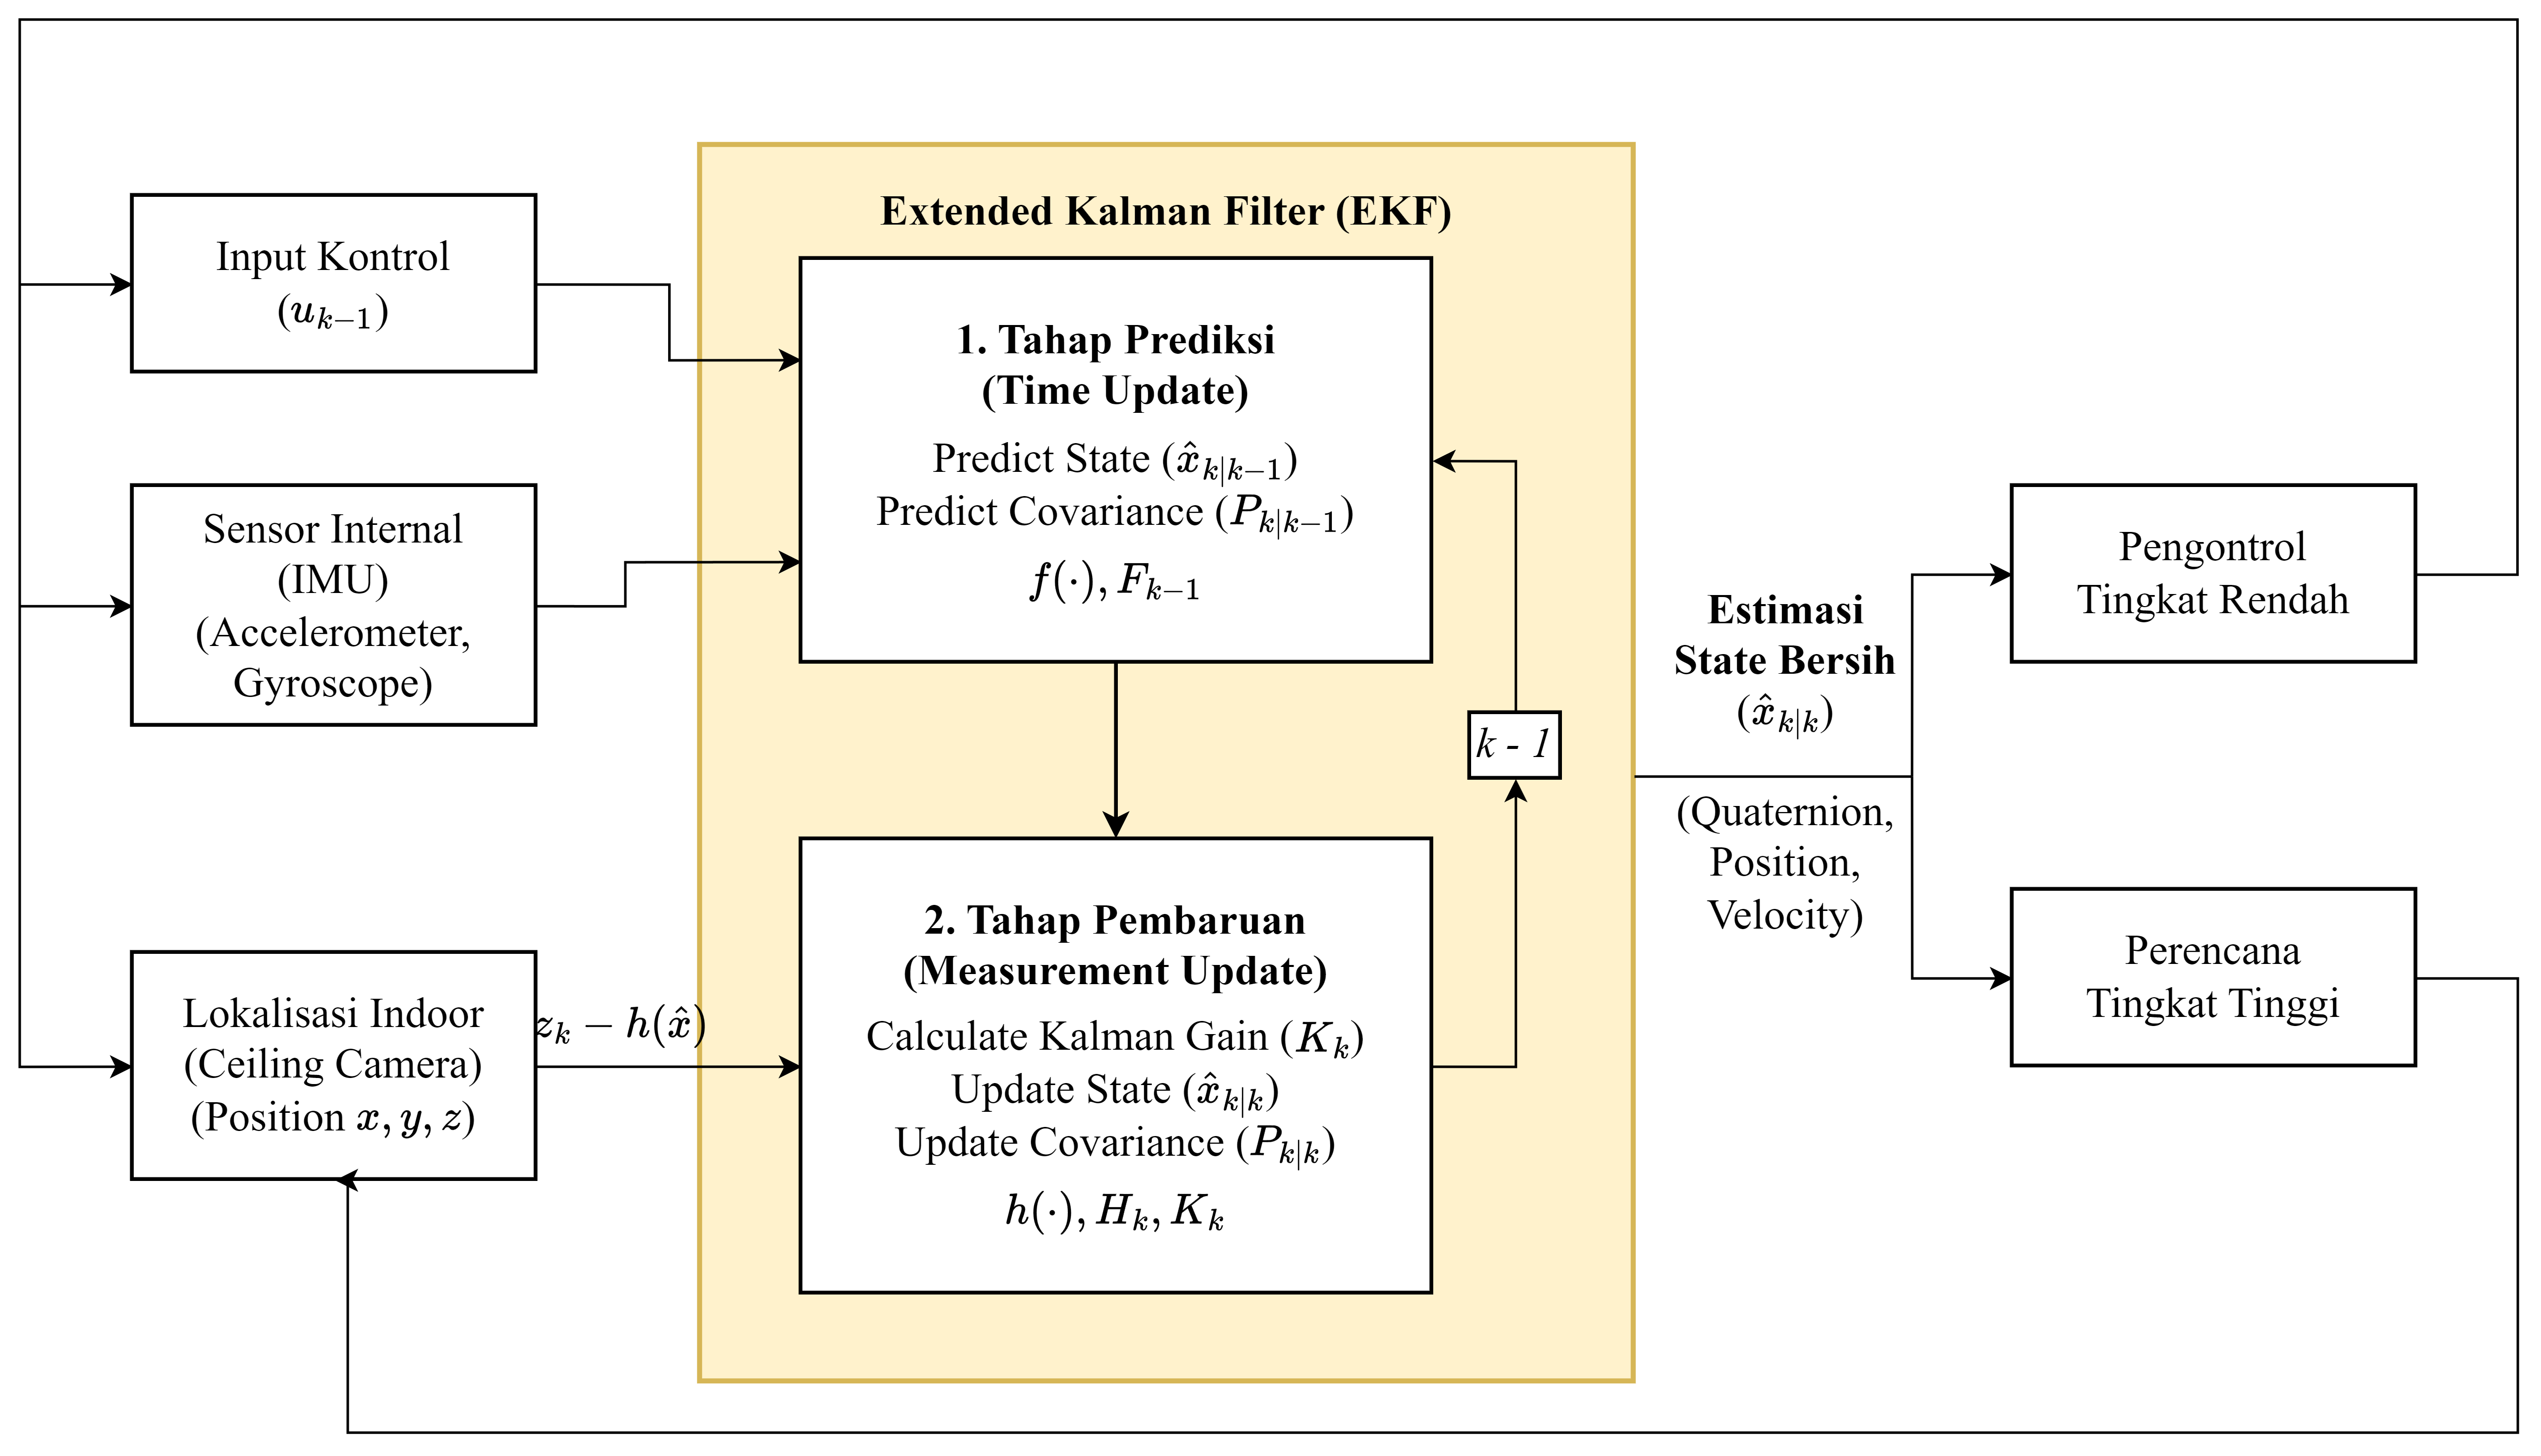
\includegraphics[width=0.9\textwidth]{figures/ekf_diagram.png}
    \caption{Arsitektur fusi sensor menggunakan \textit{Extended Kalman Filter} (EKF) untuk estimasi \textit{state} pada lingkungan \textit{indoor}.}
    \label{fig:ekf_diagram}
\end{figure}

\section{Pengontrol Tingkat Rendah (\textit{Low-Level Controller})}

Untuk stabilisasi masing-masing agen secara individu, digunakan arsitektur kontrol \textit{Proportional-Integral-Derivative} (PID) kaskade \cite{johnBobzwikQuadcopter_SimCon2025}. Struktur \textit{multi-loop} ini bertugas menerjemahkan titik referensi (\textit{setpoint}) posisi abstrak dari perencana tingkat tinggi (\textit{high-level planner}) menjadi komando motor yang konkret. Seperti yang diilustrasikan pada diagram aliran sinyal di Gambar~\ref{fig:low_level_controller}, Perencana Tingkat Tinggi memberikan posisi referensi ($x_{\mathrm{ref}}, y_{\mathrm{ref}}, z_{\mathrm{ref}}$), akselerasi referensi umpan-maju atau \textit{feedforward} ($a_{x\mathrm{ref}}, a_{y\mathrm{ref}}, a_{z\mathrm{ref}}$), serta referensi \textit{yaw} dan laju \textit{yaw} ($\psi_{\mathrm{ref}}$ dan $\dot{\psi}_{\mathrm{ref}}$).

Proses kontrol dimulai pada kalang translasi bagian luar (\textit{outer translation loops}). Pertama, Pengontrol P Posisi menghitung referensi kecepatan ($v_{x\mathrm{ref}}, v_{y\mathrm{ref}}, v_{z\mathrm{ref}}$) berdasarkan galat (\textit{error}) pelacakan posisi. Selanjutnya, Pengontrol PID Kecepatan menggunakan referensi kecepatan terhitung tersebut, kecepatan aktual terukur, dan akselerasi referensi \textit{feedforward} untuk mengkalkulasi komponen gaya dorong arah (\textit{directional thrust}) yang dibutuhkan ($T_x, T_y, T_z$).

Komponen gaya dorong ini kemudian diteruskan ke blok Konversi Gaya Dorong ke Sikap (\textit{Thrust to Attitude}). Menggunakan gaya dorong arah dan referensi \textit{yaw} ($\psi_{\mathrm{ref}}$), blok ini menghitung total gaya dorong skalar $T = \sqrt{T_x^2 + T_y^2 + T_z^2}$ (yang dirutekan langsung ke \textit{Mixer}) dan orientasi target dalam bentuk \textit{quaternion} ($q_{w\mathrm{des}}, q_{x\mathrm{des}}, q_{y\mathrm{des}}, q_{z\mathrm{des}}$).

Kalang rotasi bagian dalam (\textit{inner rotational loops}) kemudian bertugas melacak orientasi yang diinginkan ini. Pengontrol P Sikap membandingkan \textit{quaternion} target dengan sikap (\textit{attitude}) aktual terukur untuk menghasilkan laju sudut (\textit{angular rates}) yang diinginkan ($\omega_{\phi\mathrm{des}}, \omega_{\theta\mathrm{des}}, \omega_{\psi\mathrm{des}}$). Setelah itu, Pengontrol PD Laju (\textit{Rate}) menggunakan referensi laju sudut tersebut, laju sudut aktual, dan laju referensi \textit{yaw feedforward} ($\dot{\psi}_{\mathrm{ref}}$) untuk menghasilkan torsi kontrol akhir ($\tau_{\phi}, \tau_{\theta}, \tau_{\psi}$). Pada apihaknya, blok \textit{Mixer} mengalokasikan total gaya dorong skalar $T$ dan torsi kontrol untuk mendeduksi sinyal kontrol spesifik ($u_{M1}, u_{M2}, u_{M3}, u_{M4}$) yang dibutuhkan oleh dinamika aktuator motor.

\begin{figure}[htbp]
    \centering
    \makebox[\linewidth][c]{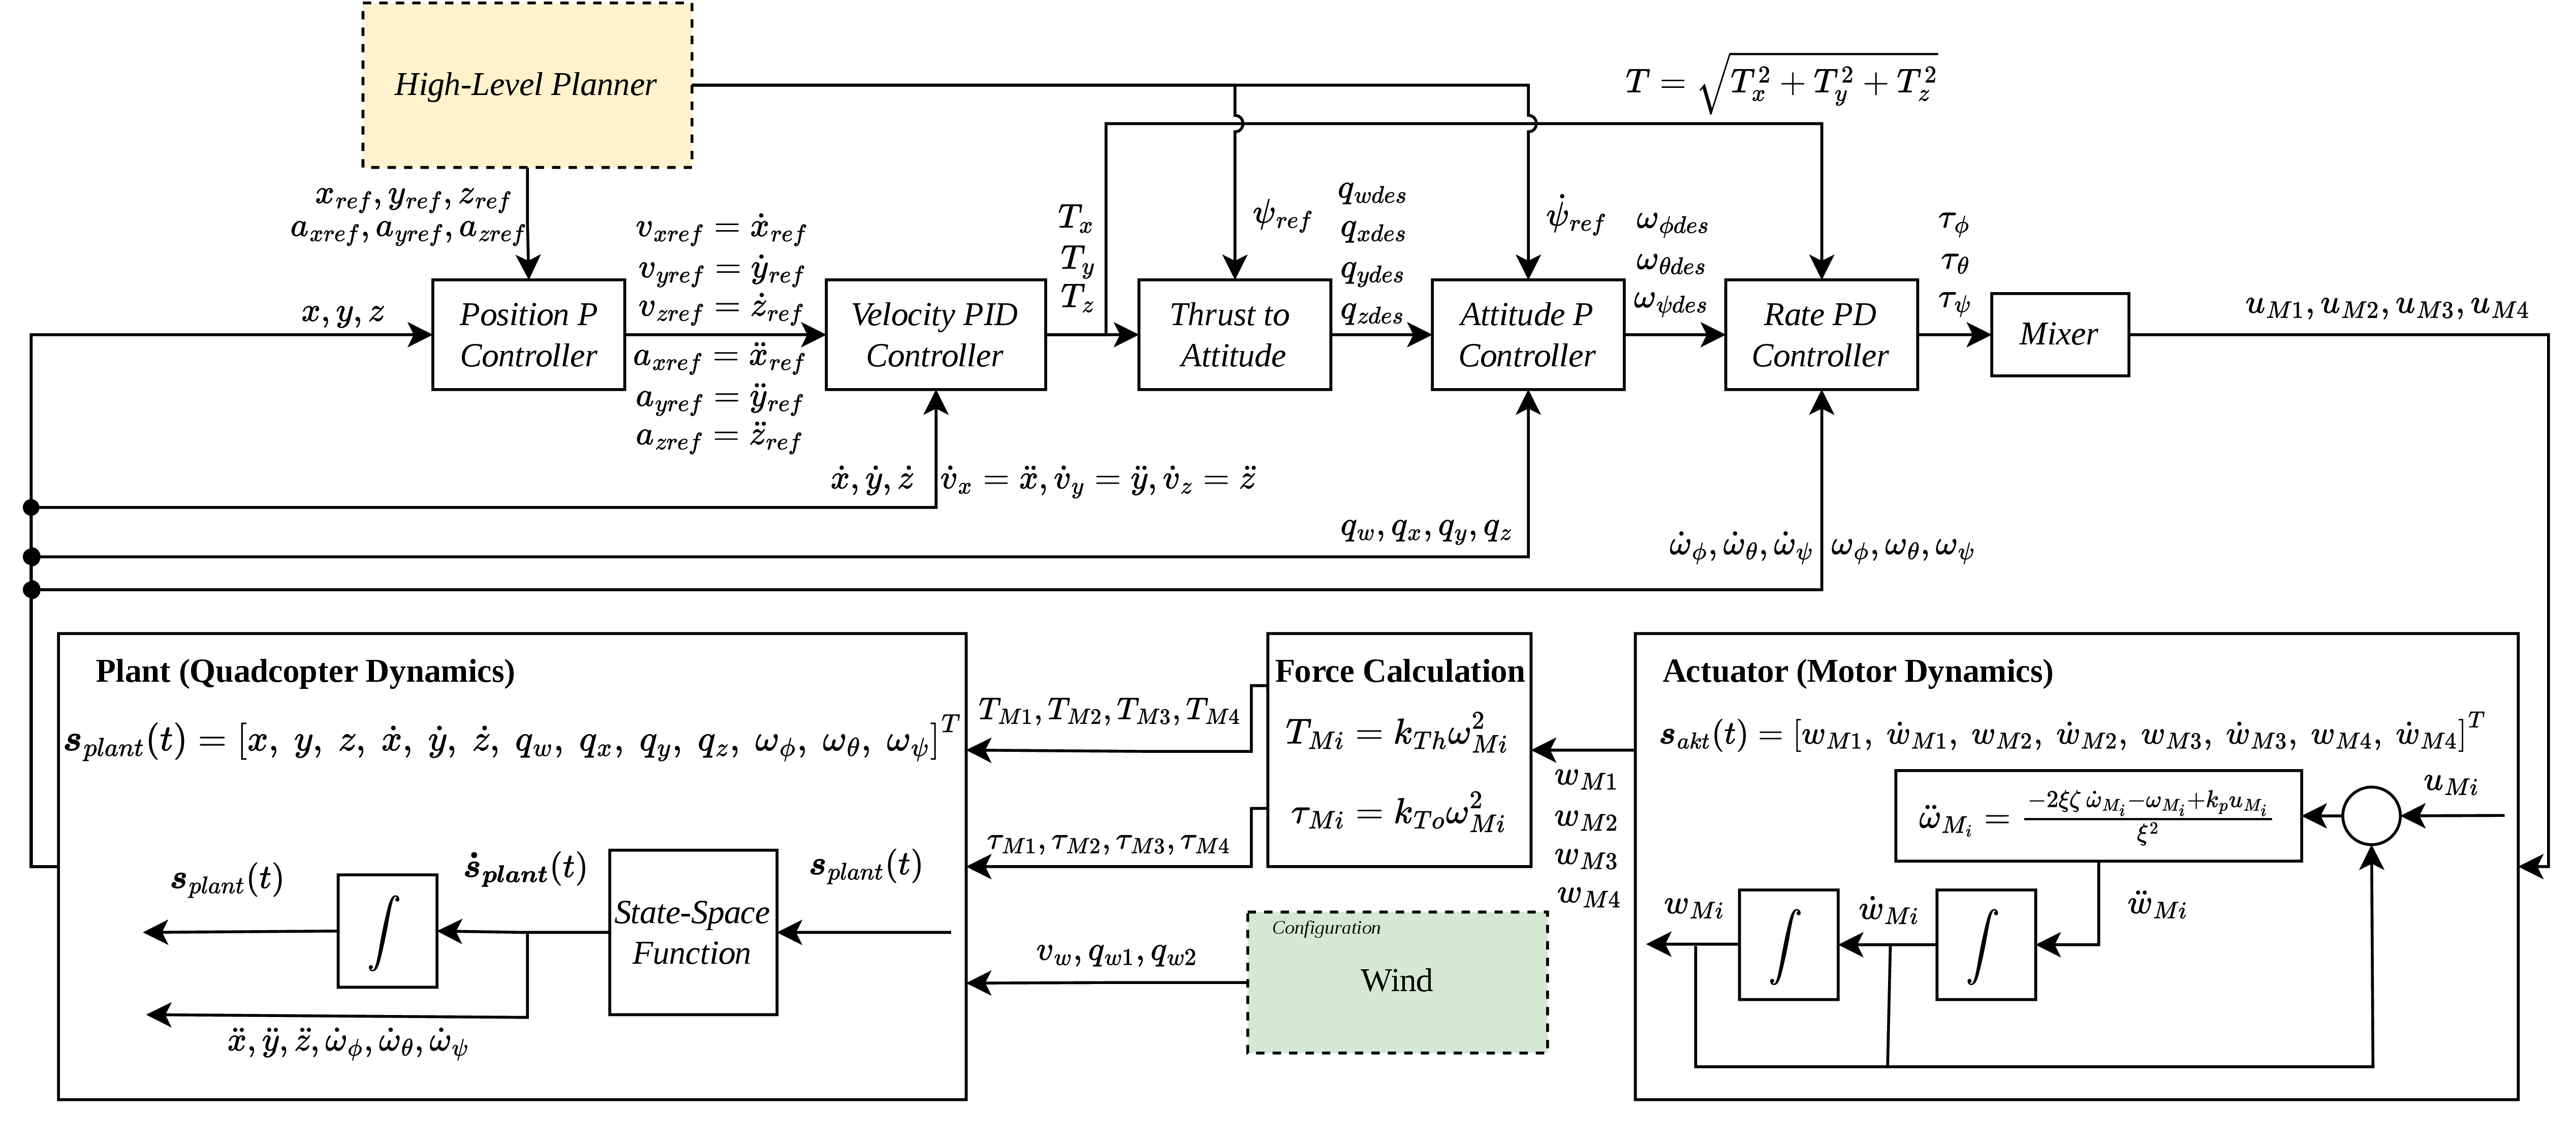
\includegraphics[width=1.2\linewidth]{figures/low_level_controller.png}}
    \caption{Arsitektur detail dari pengontrol tingkat rendah, mengilustrasikan kalang kontrol kaskade dari \textit{setpoint} posisi hingga alokasi komando motor.}
    \label{fig:low_level_controller}
\end{figure}

Sementara pengontrol tingkat rendah memastikan stabilitas pergerakan dasar masing-masing agen secara individu, perencana tingkat tinggi bertanggung jawab atas perilaku kolektif yang cerdas dari seluruh kawanan. Desain detail dari perencana ini, yang merupakan inti dari strategi kontrol formasi adaptif yang diusulkan, disajikan pada sub-bab berikutnya.

\section{Perencana Tingkat Tinggi (\textit{High-Level Planner})}
Perencana tingkat tinggi (\textit{high-level planner}) berfungsi untuk menghasilkan referensi gerak bagi setiap quadcopter berdasarkan tujuan misi, kondisi formasi, dan informasi lingkungan. Keluaran utama dari blok ini adalah posisi atau kecepatan referensi yang kemudian dikirimkan ke pengontrol tingkat rendah agar dapat diterjemahkan menjadi perintah sikap, gaya dorong, dan sinyal motor.

Arsitektur perencana tingkat tinggi ini sudah dimodifikasi dari algoritma yang dibuat oleh Bui \textit{et al.} dapat dilihat pada Gambar~\ref{fig:high_level_planner} \cite{buiEventbasedReconfigurationControl2025, PerancanganSistemKendali}. Diagram tersebut memperlihatkan bahwa masukan sistem berupa parameter misi, posisi agen, posisi rintangan, dan konfigurasi formasi diproses oleh beberapa blok utama, yaitu mesin \textit{state}, modul penghindaran tabrakan, penjagaan formasi, navigasi menuju tujuan, serta mekanisme rekonfigurasi berbasis kejadian. Hasil dari proses ini adalah referensi gerak yang bersifat adaptif, sehingga kawanan dapat mempertahankan formasi pada ruang terbuka dan menyesuaikan konfigurasi ketika menghadapi ruang sempit atau kondisi lingkungan yang berubah.

\begin{figure}[htbp]
    \centering
    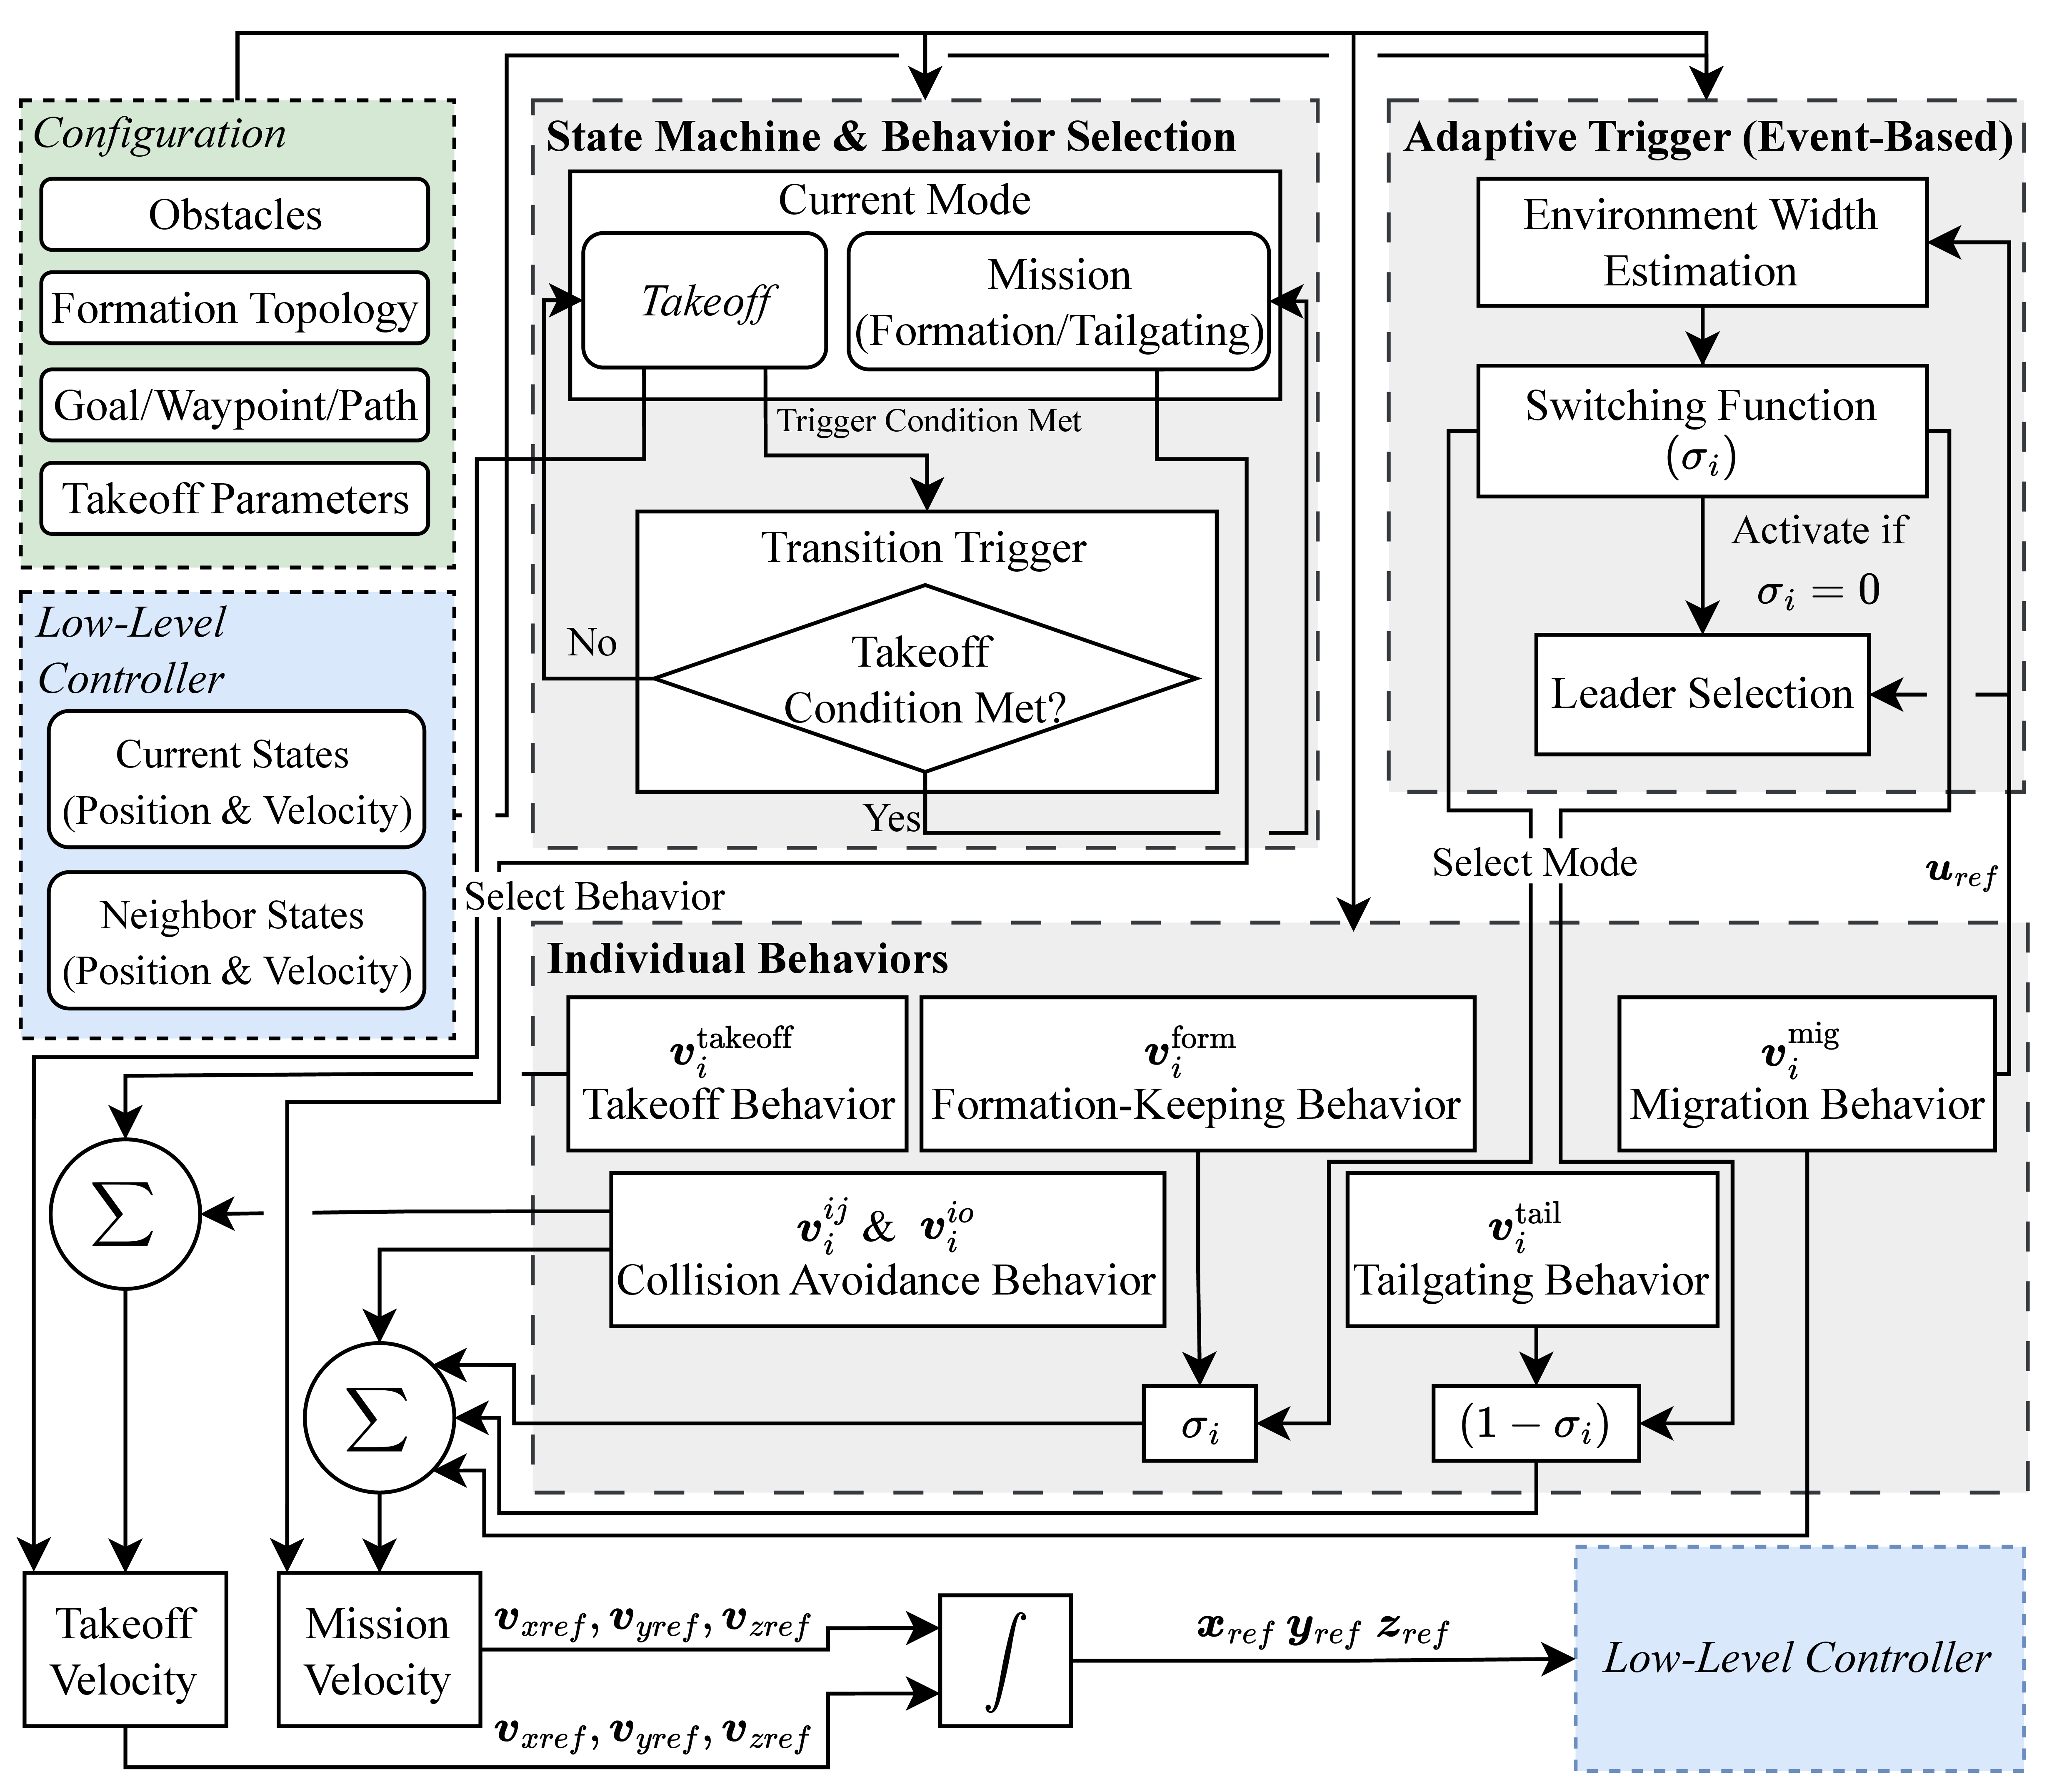
\includegraphics[width=0.8\textwidth]{figures/high_level_planner.png}
    \caption{Arsitektur perencana tingkat tinggi untuk kontrol formasi adaptif dan terdesentralisasi}
    \label{fig:high_level_planner}
\end{figure}

Dengan struktur pada Gambar~\ref{fig:high_level_planner}, proses pengambilan keputusan dilakukan pada level perencanaan, sedangkan stabilisasi gerak tetap ditangani oleh pengontrol tingkat rendah. Pemisahan ini membuat sistem lebih modular: perencana tingkat tinggi fokus pada koordinasi kawanan, sementara pengontrol tingkat rendah memastikan setiap quadcopter mampu mengikuti referensi yang diberikan secara stabil.

% ==========================================
% BAB III METODOLOGI DAN RENCANA PELAKSANAAN
% ==========================================
\chapter{METODOLOGI DAN RENCANA PELAKSANAAN}

\section{Metodologi Penelitian}
Penelitian ini dilaksanakan melalui pendekatan sistematis yang mencakup perancangan arsitektur, implementasi perangkat keras dan lunak, pengujian simulasi hibrida, hingga eksperimen penerbangan nyata dalam lingkungan \textit{indoor}. Secara keseluruhan, metodologi penelitian ini dibagi ke dalam lima fase utama yang saling berkesinambungan. Alur kerja penelitian secara lengkap diilustrasikan pada diagram alir pada Gambar~\ref{fig:diagram_metodologi}.

\begin{figure}[htbp]
    \centering
    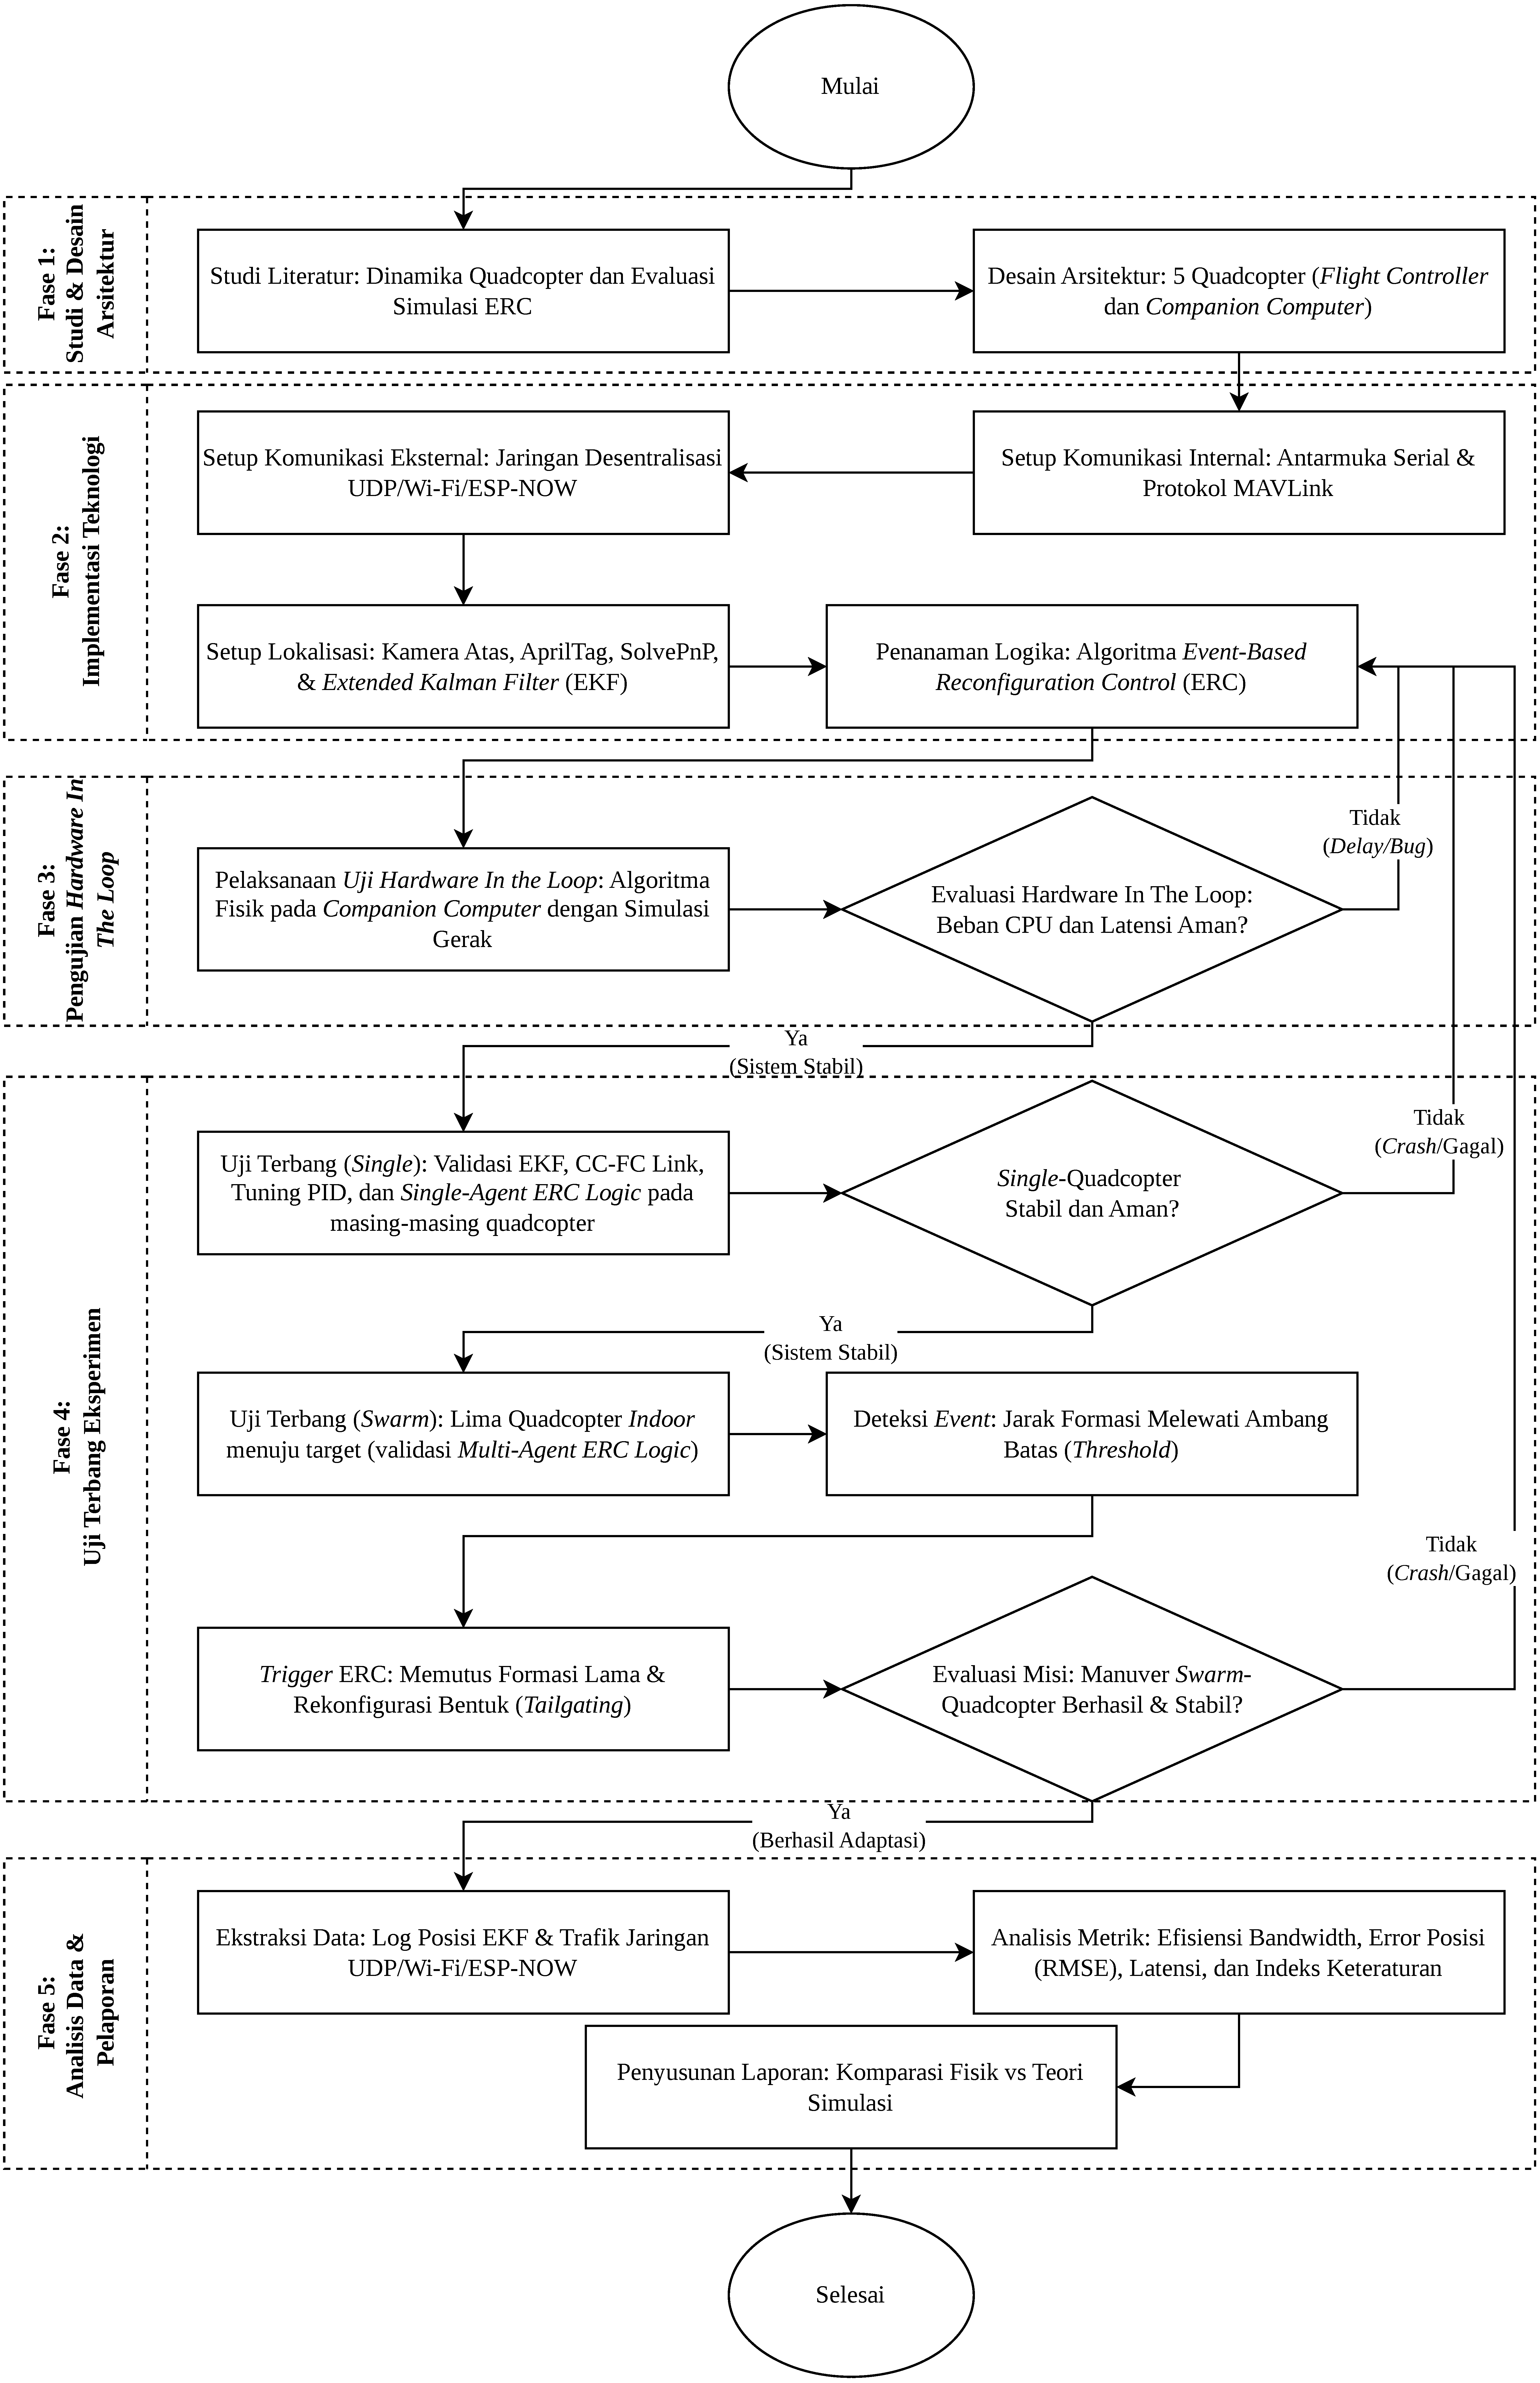
\includegraphics[width=\textwidth]{figures/metodologi_tesis.pdf}
    \caption{Diagram alir metodologi penelitian untuk implementasi kontrol formasi desentralisasi pada kawanan quadcopter.}
    \label{fig:diagram_metodologi}
\end{figure}

\subsection{Fase 1: Studi dan Desain Arsitektur}
Fase pertama difokuskan pada pematangan konsep teoritis dan perancangan arsitektur sistem. Tahapan ini diawali dengan studi literatur mendalam mengenai dinamika quadcopter dan evaluasi simulasi dari algoritma \textit{Event-Based Reconfiguration Control} (ERC). Berdasarkan landasan teoritis tersebut, dilakukan desain arsitektur perangkat keras untuk lima buah agen quadcopter. Desain ini menetapkan pembagian tugas komputasi secara hierarkis antara \textit{Flight Controller} (sebagai pengontrol tingkat rendah) dan \textit{Companion Computer} (sebagai perencana tingkat tinggi).

\subsection{Fase 2: Implementasi Teknologi}
Fase kedua merupakan tahap perakitan dan konfigurasi sistem secara menyeluruh, yang mencakup:
\begin{itemize}
    \item \textbf{Setup Komunikasi Eksternal:} Membangun jaringan komunikasi terdesentralisasi antar-wahana menggunakan modul Wi-Fi/ESP-NOW dengan protokol UDP.
    \item \textbf{Setup Komunikasi Internal:} Mengkonfigurasi antarmuka serial (UART) untuk menjembatani komunikasi data berformat MAVLink antara \textit{Companion Computer} dan \textit{Flight Controller}.
    \item \textbf{Setup Lokalisasi:} Mengintegrasikan sistem penentuan posisi \textit{indoor} (seperti UWB atau OptiTrack) dan mengimplementasikan \textit{Extended Kalman Filter} (EKF) untuk fusi data sensor.
    \item \textbf{Penanaman Logika:} Menginisialisasi dan menanamkan (\textit{embedding}) program algoritma ERC dan IAPF\label{abbr:iapf} ke dalam unit \textit{Companion Computer} masing-masing agen.
\end{itemize}

\subsection{Fase 3: Pengujian \textit{Hardware-In-The-Loop} (HITL\label{abbr:hitl})}
Sebelum diterbangkan, sistem menjalani pengujian \textit{Hardware-In-The-Loop} (HITL). Pada tahap ini, algoritma fisik yang telah ditanamkan pada \textit{Companion Computer} diuji menggunakan data umpan balik dari simulator gerak virtual. Pengujian ini bertujuan untuk mengevaluasi kelayakan beban kerja CPU dan memastikan latensi komputasi berada dalam batas aman. Jika terdeteksi adanya \textit{delay} atau \textit{bug} yang menyebabkan sistem tidak stabil, proses akan diulang kembali ke tahap penanaman logika untuk dilakukan perbaikan kode.

\subsection{Fase 4: Uji Terbang Eksperimen}
Fase ini merupakan validasi fisik di arena penerbangan \textit{indoor}, yang dieksekusi secara bertahap:
\begin{enumerate}
    \item \textbf{Uji Terbang Tunggal (\textit{Single-Agent}):} Melibatkan satu quadcopter untuk memvalidasi kinerja EKF, stabilitas tautan komunikasi MAVLink, \textit{tuning} parameter PID, dan eksekusi logika ERC agen tunggal. Pengujian kawanan hanya akan dilanjutkan apabila agen tunggal terbukti stabil dan aman.
    \item \textbf{Uji Terbang Kawanan (\textit{Swarm}):} Melibatkan kelima quadcopter yang terbang bersama menuju target tujuan. Tahap ini menguji logika multi-agen, di mana sistem harus mampu mendeteksi \textit{event} atau kejadian kritis (misalnya jarak rintangan atau formasi melewati ambang batas toleransi), dan memicu algoritma ERC untuk memutus keutuhan formasi lama guna merekonfigurasi bentuk kawanan menjadi formasi mengekor (\textit{tailgating}).
\end{enumerate}

\subsection{Fase 5: Analisis Data dan Pelaporan}
Fase terakhir dilakukan setelah eksekusi eksperimen berhasil dilewati. Data penerbangan diekstraksi dari \textit{log} sistem, yang mencakup rekaman data posisi estimasi dari EKF, serta rekaman kepadatan trafik jaringan komunikasi (UDP\label{abbr:udp}/Wi-Fi/ESP-NOW). Data empiris ini kemudian dianalisis untuk memvalidasi keberhasilan respons manuver adaptif sistem dan mengukur kinerja latensi jaringan desentralisasinya, yang pada akhirnya disusun ke dalam dokumen laporan atau tesis akhir.

\section{Rencana Pelaksanaan}
Pelaksanaan penelitian ini direncanakan secara sistematis mencakup tahap perancangan, implementasi perangkat keras dan lunak, pengujian komputasi, hingga eksperimen penerbangan fisik dan evaluasi data. Seluruh rangkaian kegiatan ini disusun agar target penelitian dapat dicapai secara terstruktur, efisien, dan memenuhi standar keselamatan pengujian wahana udara.

\subsection{Lokasi Pelaksanaan}
Seluruh rangkaian penelitian akan dilaksanakan di Pusat Teknologi Instrumentasi dan Otomasi (PTIO\label{abbr:ptio}), Gedung Pusat Antar Universitas (PAU) Lantai 8, Institut Teknologi Bandung. Kegiatan yang dilakukan di lokasi ini mencakup perakitan wahana (\textit{hardware assembly}), pemrograman \textit{companion computer}, pengujian \textit{Hardware-In-The-Loop} (HITL), serta eksperimen uji terbang kawanan quadcopter di lingkungan dalam ruangan (\textit{indoor}).

\subsection{Alat dan Bahan}
Pelaksanaan penelitian ini membutuhkan beberapa komponen pendukung untuk merealisasikan sistem navigasi kawanan quadcopter, terutama pada aspek persepsi rintangan, lokalisasi spasial, pemrosesan visi komputer, dan keselamatan pengujian.
Perangkat utama yang digunakan meliputi sensor ultrasonik sebagai pendeteksi jarak lateral diagonal, kamera sudut lebar laju tinggi (60 FPS) yang dipasang di langit-langit beserta penanda visual (\textit{AprilTag}) sebagai sistem lokalisasi \textit{indoor}, serta perlengkapan keselamatan untuk mendukung eksperimen di lingkungan \textit{indoor}.

Pemilihan sensor ultrasonik dilakukan karena kebutuhan penelitian berfokus pada deteksi jarak lateral terhadap rintangan secara ekonomis dan ringkas.
Jumlah sensor ultrasonik disesuaikan dengan konfigurasi lima agen quadcopter, yaitu dua sensor pada setiap agen (dipasang secara diagonal dengan sudut $\theta = 45^\circ$) untuk memantau sisi kiri dan kanan wahana.
Selain itu, penanda visual \textit{AprilTag} dicetak pada stiker bercorak \textit{matte} dan ditempelkan pada alas akrilik tipis di atas bodi wahana guna memastikan estimasi pose 3D oleh kamera atas berjalan stabil.
Rincian alat, bahan, kuantitas, serta estimasi biaya pengadaan komponen utama penelitian dirangkum pada Tabel~\ref{tab:alat_bahan}.

\begin{table}[htbp]
    \centering
    \caption{Rencana Anggaran Biaya (RAB) Komponen Utama Wahana}
    \label{tab:alat_bahan}
    \begingroup
    \small
    \setlength{\tabcolsep}{3pt}
    \renewcommand{\arraystretch}{1.3}
    \begin{tabularx}{\textwidth}{|c|X|>{\centering\arraybackslash}p{1.9cm}|>{\raggedleft\arraybackslash}p{2.4cm}|>{\raggedleft\arraybackslash}p{2.3cm}|}
        \hline
        \rowcolor{gray!20}
        \thead{No} & \thead{Komponen} & \thead{Kuantitas} & \thead{Harga Satuan\\(Rp)} & \thead{Harga Total\\(Rp)} \\ \hline
        1 & Sensor Ultrasonik (HC-SR04) & 10 & 20.000 & 200.000 \\ \hline
        2 & Kamera Atas 60 FPS (\textit{Ceiling Camera}) & 1 & 1.500.000 & 1.500.000 \\ \hline
        3 & Penanda Visual \textit{AprilTag} + Akrilik 1mm & 5 Set & 20.000 & 100.000 \\ \hline
        4 & Kabel USB Extension 10m + \textit{Ceiling Mount} & 1 Set & 150.000 & 150.000 \\ \hline
        5 & Dus sebagai rintangan & 10 & 30.000 & 300.000 \\ \hline
        6 & Alat \textit{Safety} & 1 & 500.000 & 500.000 \\ \hline
        \multicolumn{4}{|r|}{\textbf{TOTAL HARGA}} & \textbf{2.750.000} \\ \hline
    \end{tabularx}
    \endgroup
\end{table}

\textit{Catatan:} Estimasi biaya pada Tabel~\ref{tab:alat_bahan} hanya mencakup komponen tambahan yang diperlukan untuk penelitian. Komponen utama wahana seperti rangka quadcopter SpeedyBee 35, motor BLDC, ESC 4-in-1, baterai, \textit{flight controller} SpeedyBee F4 Mini, dan \textit{companion computer} (ESP32S3) diasumsikan telah tersedia sebagai bagian dari fasilitas laboratorium PTIO ITB atau perangkat penelitian yang telah ada.

\textit{Catatan:} Estimasi biaya pada Tabel~\ref{tab:alat_bahan} hanya mencakup komponen tambahan yang diperlukan untuk penelitian. Komponen utama wahana seperti rangka quadcopter SpeedyBee 35, motor BLDC, ESC 4-in-1, baterai, \textit{flight controller} SpeedyBee F4 Mini, dan \textit{companion computer} (ESP32S3) diasumsikan telah tersedia sebagai bagian dari fasilitas laboratorium PTIO ITB atau perangkat penelitian yang telah ada.

\subsection{Biaya}
Berdasarkan kebutuhan alat dan bahan yang telah diidentifikasi, total estimasi biaya pengadaan komponen utama penelitian adalah sebesar Rp4.850.000. Porsi biaya terbesar berasal dari pengadaan modul UWB, yaitu sekitar Rp3,75 juta. Modul tersebut dibutuhkan pada setiap agen quadcopter untuk mendukung proses lokalisasi. Komponen lain, seperti sensor ultrasonik, kamera sudut lebar, dus sebagai rintangan, dan perlengkapan keselamatan, digunakan untuk mendukung pengujian persepsi lingkungan serta menjaga keamanan selama eksperimen berlangsung.

Estimasi biaya tersebut bersifat awal dan dapat berubah menyesuaikan ketersediaan komponen, harga pasar, serta kebutuhan teknis tambahan pada tahap implementasi. Namun demikian, daftar biaya ini memberikan gambaran kebutuhan minimum yang diperlukan agar sistem persepsi, lokalisasi, dan pengujian eksperimen kawanan quadcopter dapat dilaksanakan secara memadai.

\subsection{Jadwal Pelaksanaan}
Penelitian ini direncanakan berlangsung selama sembilan bulan, dimulai pada bulan Agustus 2026 hingga April 2027. Rangkaian kegiatan ini mencakup seluruh tahap metodologi, mulai dari studi literatur dan perancangan awal, dilanjutkan dengan tahap perakitan dan konfigurasi sistem (Agustus--November 2026). Setelah perangkat keras dan lunak terintegrasi, fokus penelitian akan beralih pada pengujian \textit{Hardware-In-The-Loop} (HITL) dan uji terbang secara berkala dari akhir tahun hingga kuartal pertama tahun berikutnya. Alokasi waktu satu bulan penuh di akhir periode dikhususkan untuk ekstraksi data penerbangan, analisis metrik kinerja sistem, dan penyusunan dokumen laporan.

Rincian estimasi jadwal pelaksanaan kegiatan secara spesifik dijabarkan dalam bentuk \textit{Gantt chart} pada Tabel~\ref{tab:jadwal_pelaksanaan}.

\begin{table}[htbp]
    \centering
    \caption{Jadwal Pelaksanaan Penelitian Agustus 2026--April 2027}
    \label{tab:jadwal_pelaksanaan}
    \renewcommand{\arraystretch}{1.3}
    \resizebox{\textwidth}{!}{%
    \begin{tabular}{|c|p{11.5cm}|c|c|c|c|c|c|c|c|c|}
        \hline
        \rowcolor{gray!20}
        & & \multicolumn{5}{c|}{\textbf{2026}} & \multicolumn{4}{c|}{\textbf{2027}} \\ \cline{3-11}
        \rowcolor{gray!20}
        & & \multicolumn{9}{c|}{\textbf{Bulan}} \\ \cline{3-11}
        \rowcolor{gray!20}
        % Perintah multirow dipindah ke baris terakhir dengan indeks -3
        \multirow{-3}{*}{\textbf{No}} & \multirow{-3}{=}{\centering\textbf{Detail Kegiatan}} & \textbf{8} & \textbf{9} & \textbf{10} & \textbf{11} & \textbf{12} & \textbf{1} & \textbf{2} & \textbf{3} & \textbf{4} \\ \hline
        1 & Studi Literatur: Dinamika Quadcopter dan Evaluasi Simulasi ERC & \cellcolor{gray!70} & \cellcolor{gray!70} & \cellcolor{gray!70} & \cellcolor{gray!70} & \cellcolor{gray!70} & \cellcolor{gray!70} & \cellcolor{gray!70} & \cellcolor{gray!70} & \cellcolor{gray!70} \\ \hline
        2 & Desain Arsitektur: 5 Quadcopter (Flight Controller dan Companion Computer) & \cellcolor{gray!70} & & & & & & & & \\ \hline
        3 & Setup Komunikasi Internal: Antarmuka Serial \& Protokol MAVLink\label{abbr:mavlink} & & \cellcolor{gray!70} & \cellcolor{gray!70} & & & & & & \\ \hline
        4 & Setup Komunikasi Eksternal: Jaringan Desentralisasi UDP/Wi-Fi/ESP-NOW & & \cellcolor{gray!70} & \cellcolor{gray!70} & & & & & & \\ \hline
        5 & Setup Lokalisasi: Integrasi OptiTrack/UWB \& Extended Kalman Filter (EKF) & & \cellcolor{gray!70} & \cellcolor{gray!70} & & & & & & \\ \hline
        6 & Penanaman Logika: Algoritma Event-Based Reconfiguration Control (ERC) & & \cellcolor{gray!70} & \cellcolor{gray!70} & \cellcolor{gray!70} & & & & & \\ \hline
        7 & Pelaksanaan Uji Hardware In the Loop: Algoritma Fisik pada Companion Computer dengan Simulasi Gerak & & & & \cellcolor{gray!70} & \cellcolor{gray!70} & & & & \\ \hline
        8 & Uji Terbang (Single): Validasi EKF, CC-FC Link, Tuning PID\label{abbr:pid}, dan Single-Agent ERC Logic pada masing-masing quadcopter & & & & \cellcolor{gray!70} & \cellcolor{gray!70} & & & & \\ \hline
        9 & Uji Terbang (Swarm): Lima Quadcopter Indoor menuju target (validasi Multi-Agent ERC Logic) & & & & & \cellcolor{gray!70} & \cellcolor{gray!70} & \cellcolor{gray!70} & \cellcolor{gray!70} & \\ \hline
        10 & Deteksi Event: Jarak Formasi Melewati Ambang Batas (Threshold) & & & & & \cellcolor{gray!70} & \cellcolor{gray!70} & \cellcolor{gray!70} & \cellcolor{gray!70} & \\ \hline
        11 & Trigger ERC: Memutus Formasi Lama \& Rekonfigurasi Bentuk (Tailgating) & & & & & \cellcolor{gray!70} & \cellcolor{gray!70} & \cellcolor{gray!70} & \cellcolor{gray!70} & \\ \hline
        12 & Ekstraksi Data: Log Posisi EKF \& Trafik Jaringan UDP/Wi-Fi/ESP-NOW & & & & & & & & & \cellcolor{gray!70} \\ \hline
        13 & Analisis Metrik: Efisiensi Bandwidth, Error Posisi (RMSE\label{abbr:rmse}), Latensi, dan Indeks Keteraturan & & & & & & & & & \cellcolor{gray!70} \\ \hline
        14 & Penyusunan Laporan: Komparasi Fisik vs Teori Simulasi & & & & & & & & & \cellcolor{gray!70} \\ \hline
    \end{tabular}%
    }
\end{table}

% ==========================================
% BAB IV PENUTUP
% ==========================================
\chapter{PENUTUP}
Proposal tesis ini disusun sebagai landasan komprehensif dalam pelaksanaan penelitian tesis yang berjudul ``Implementasi Fisik dan Evaluasi \textit{Event-Based Reconfiguration Control} pada Sistem Formasi Adaptif Terdesentralisasi Kawanan \textit{Quadcopter} di Ruang Sempit''. Penyusunan proposal ini telah dilakukan dengan mempertimbangkan berbagai tinjauan teoretis dan rancangan teknis yang kuat guna mendukung kelancaran eksperimen pada platform fisik. Melalui dokumen ini, diharapkan seluruh rencana penelitian dapat tergambar secara terstruktur dan menjadi pedoman yang jelas dalam setiap tahapan implementasi yang akan dilakukan. Pada akhirnya, semoga proposal ini dapat mendukung kelancaran penelitian dari awal hingga akhir, serta mencapai tujuan kontribusi keilmuan yang telah ditetapkan.

% ==========================================
% DAFTAR PUSTAKA (MENGGUNAKAN BERKAS EKSTERNAL)
% ==========================================
\clearpage
\renewcommand{\bibname}{DAFTAR PUSTAKA} % Mengubah judul bawaan menjadi "DAFTAR PUSTAKA".
\addcontentsline{toc}{chapter}{DAFTAR PUSTAKA} % Memasukkan daftar pustaka ke dalam daftar isi.

% Menentukan gaya tampilan daftar pustaka.
\bibliographystyle{ieeetr}

% Memuat basis data pustaka dari berkas references.bib.
\bibliography{references}

\end{document}